\documentclass[11pt]{report}

%using utf8
\usepackage[utf8]{inputenc}
\usepackage[english]{babel}

\usepackage[pdftex]{graphicx}

\usepackage{titlesec}

% used for appendix
\usepackage{pdfpages}

\usepackage[acronym]{glossaries}

%embed urls
\usepackage{hyperref}
\usepackage{url}

%can use blind text
\usepackage{blindtext}

%improves the caption
\usepackage[font=it]{caption}

% to remove the number from the equations.
\usepackage{amsmath}

% fix quotes
\usepackage [english]{babel}
\usepackage [autostyle, english = american]{csquotes}
\MakeOuterQuote{"}

%Removes the Chapter from each chapter headline
\titleformat{\chapter}[block]
  {\normalfont\huge\bfseries}{\thechapter.}{1em}{\Huge}

\makeglossaries
\newacronym{fca}{FCA}{Formal Concept Analysis}
\newacronym{dt}{DT}{Dynamic Taxonomy}
\newacronym{ir}{IR}{Information Retrieval}
\newacronym{dom}{DOM}{Document Object Model}
\newacronym{hci}{HCI}{Human-Computer Interaction}

\begin{document}

%%%%%%%%%%%%%%%%%%%%%%%%%%%%%%%%%%%%%%%%%
% University Assignment Title Page 
% LaTeX Template
% Version 1.0 (27/12/12)
%
% This template has been downloaded from:
% http://www.LaTeXTemplates.com
%
% Original author:
% WikiBooks (http://en.wikibooks.org/wiki/LaTeX/Title_Creation)
%
% License:
% CC BY-NC-SA 3.0 (http://creativecommons.org/licenses/by-nc-sa/3.0/)
% 
% Instructions for using this template:
% This title page is capable of being compiled as is. This is not useful for 
% including it in another document. To do this, you have two options: 
%
% 1) Copy/paste everything between \begin{document} and \end{document} 
% starting at \begin{titlepage} and paste this into another LaTeX file where you 
% want your title page.
% OR
% 2) Remove everything outside the \begin{titlepage} and \end{titlepage} and 
% move this file to the same directory as the LaTeX file you wish to add it to. 
% Then add \input{./title_page_1.tex} to your LaTeX file where you want your
% title page.
%
%%%%%%%%%%%%%%%%%%%%%%%%%%%%%%%%%%%%%%%%%

%----------------------------------------------------------------------------------------
%	PACKAGES AND OTHER DOCUMENT CONFIGURATIONS
%----------------------------------------------------------------------------------------

\begin{titlepage}

\newcommand{\HRule}{\rule{\linewidth}{0.5mm}} % Defines a new command for the horizontal lines, change thickness here

\center % Center everything on the page
 
%----------------------------------------------------------------------------------------
%	HEADING SECTIONS
%----------------------------------------------------------------------------------------

\includegraphics[width=0.15\textwidth]{./logo}\\[1cm]

\textsc{\LARGE Otto-von-Guericke University Magdeburg}\\[0.5cm] % Name of your university/college
\textsc{\large Faculty of Computer Science}\\[1.0cm] % Minor heading such as course title
\textsc{\Large Bachelor's Thesis}\\[1.0cm] % Major heading such as course name

%----------------------------------------------------------------------------------------
%	TITLE SECTION
%----------------------------------------------------------------------------------------

\HRule \\[0.5cm]
{ \huge \bfseries Interactive Visualization of Large Concept Lattices for Exploratory Search}\\[0.5cm] % Title of your document
\HRule \\[1.0cm]
 
%----------------------------------------------------------------------------------------
%	AUTHOR SECTION
%----------------------------------------------------------------------------------------

\Large \emph{Author:}\\
Johannes \textsc{Filter}\\[0.5cm]

\Large \emph{Advisors:}\\
Prof. Dr. Andreas \textsc{Nürnberger}\\
{\small Otto-von-Guericke University Magdeburg}\\[0.5cm]

Prof. Dr. Ana \textsc{García-Serrano}\\
{\small Universidad Nacional de Educación a Distancia}\\[1.0cm]

%----------------------------------------------------------------------------------------
%	DATE SECTION
%----------------------------------------------------------------------------------------

{\large \today}

\vfill % Fill the rest of the page with whitespace

\end{titlepage}

\renewcommand{\thepage}{\roman{page}}% Roman numerals for page counter

\newpage
\thispagestyle{empty}
\mbox{}

\chapter*{Abstract}
\blindtext

\newpage
\thispagestyle{empty}
\mbox{}

\chapter*{Zusammenfassung}
\blindtext

\newpage
\thispagestyle{empty}
\mbox{}

\chapter*{Acknowledgements}
\blindtext

\newpage
\thispagestyle{empty}
\mbox{}

\tableofcontents
\newpage

\printglossary[type=\acronymtype]

\newpage
\thispagestyle{empty}
\mbox{}

\chapter{Introduction}
\label{Introduction}

\renewcommand{\thepage}{\arabic{page}}
\setcounter{page}{1}

The digital revolution is affecting every part of our life. Also the humanities scholars witness a change in their work life when analog collections are digitized. They have to apply computer science methods to organize and analyze huge amount of data. The area "digital humanities" evolved during the last ten years and it can be defined as an "intersection between the humanities and information technology" \cite{Svensson2010}.\\

 The computer science department of the Universidad Nacional de Educación a Distancia (UNED) in Madrid cooperates with human scholars to conduct research in the digital humanities. In this project\footnote{\url{http://linhd.uned.es/p/proyecto-dimh}}, there work on historical maps. The maps were drawn between 1503 and 1805, digitized and are available on the web\footnote{\url{http://www.mcu.es/ccbae/es/consulta/resultados_busqueda.cmd?busq_codsecc=MCAGS}} for search. The maps have been annotated by human scholars. A example of a map is shown in Figure~\ref{figure:map} with its annotation in Figure~\ref{figure:metadata}. \\
 
\begin{figure*}[!ht]
	\centering
	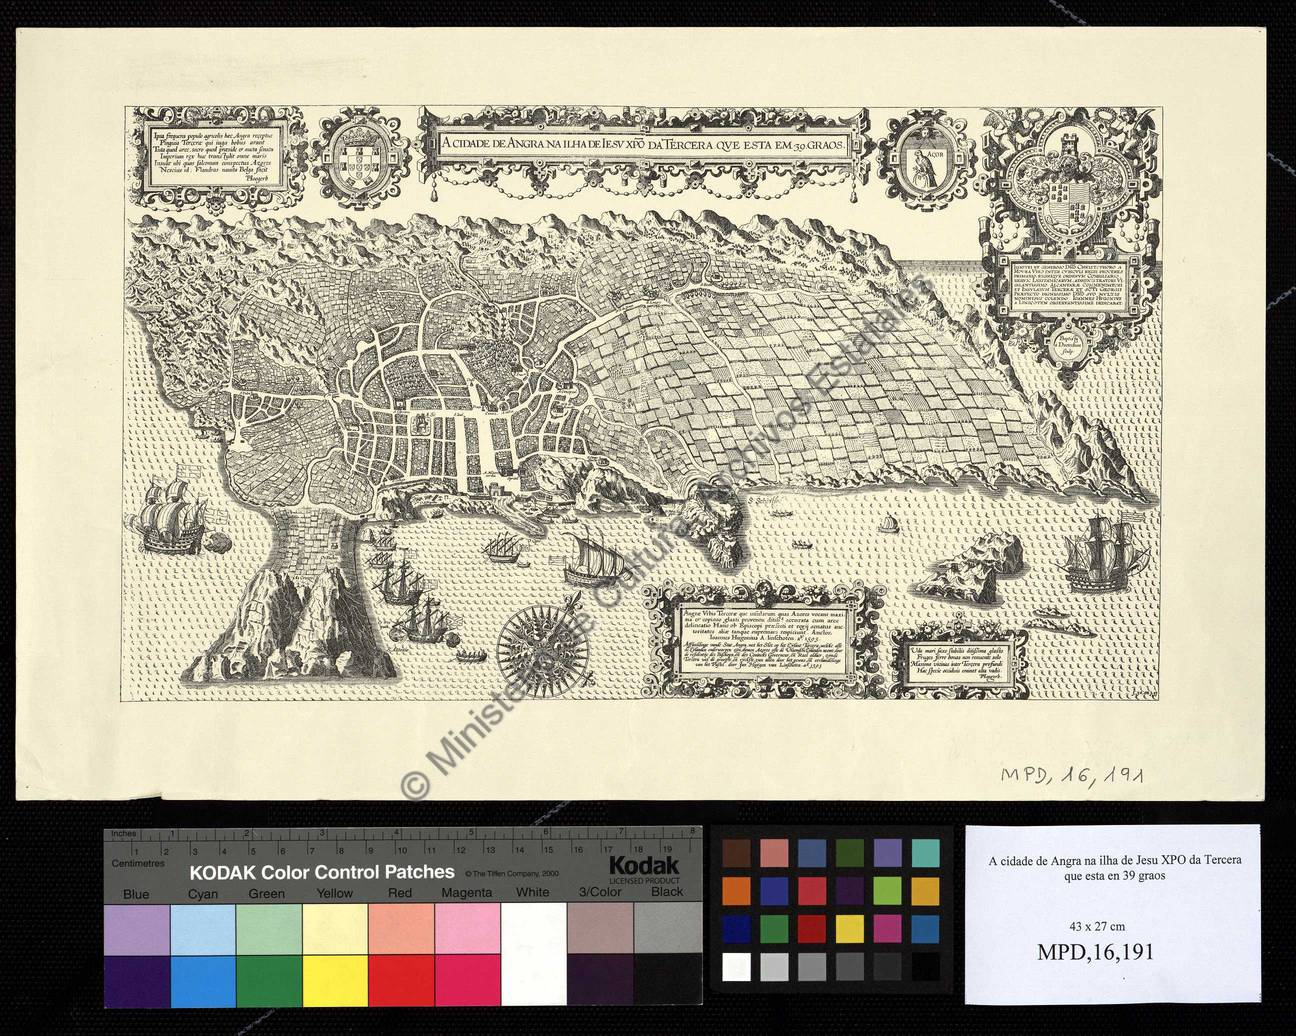
\includegraphics[width=\linewidth]{./images/map}
\caption{Digitized Map}
\label{figure:map}
\end{figure*}

\begin{figure*}[!ht]
	\centering
	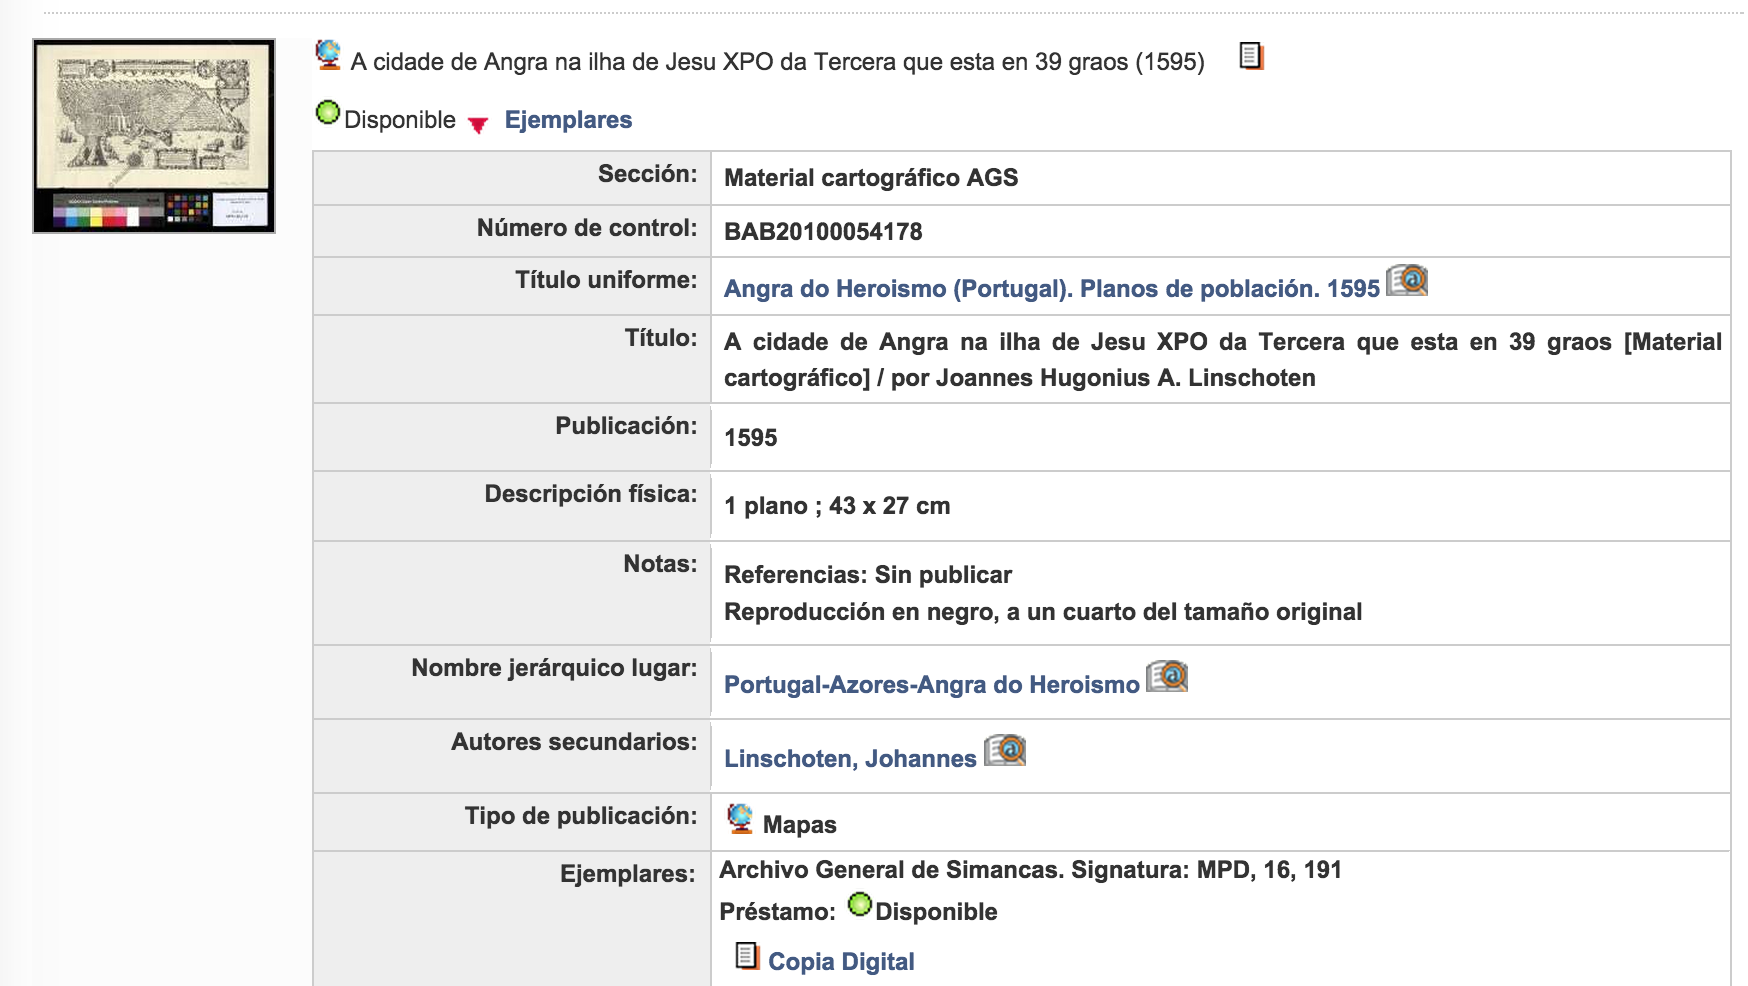
\includegraphics[width=\linewidth]{./images/metadata}
\caption{Annotation of a digitized map}
\label{figure:metadata}
\end{figure*}

To extract knowledge from the collection, the research group advocates for the use of a mathematical techniques called \acrlong{fca} \cite{Castellanos,Cigarran}. After applying this technique, the maps are organized in hierarchical structure which is called concept lattice. A concept lattice is a special form of lattice. There exist a static visualizations for lattices which is called Hasse diagram. An example of a Hasse diagram is shown in Figure~\ref{figure:hasse}. In this diagram, you can see the power set of the set $\{x,y,z\}$ and the hierarchical relationships among them. The arrows indicate if a set (the origin) is a subset another set (the destination). The nodes are layered in regard to number of elements in a set. The node with the most items is in the top and the empty set is in the bottom. \\

\begin{figure*}[!ht]
	\centering
	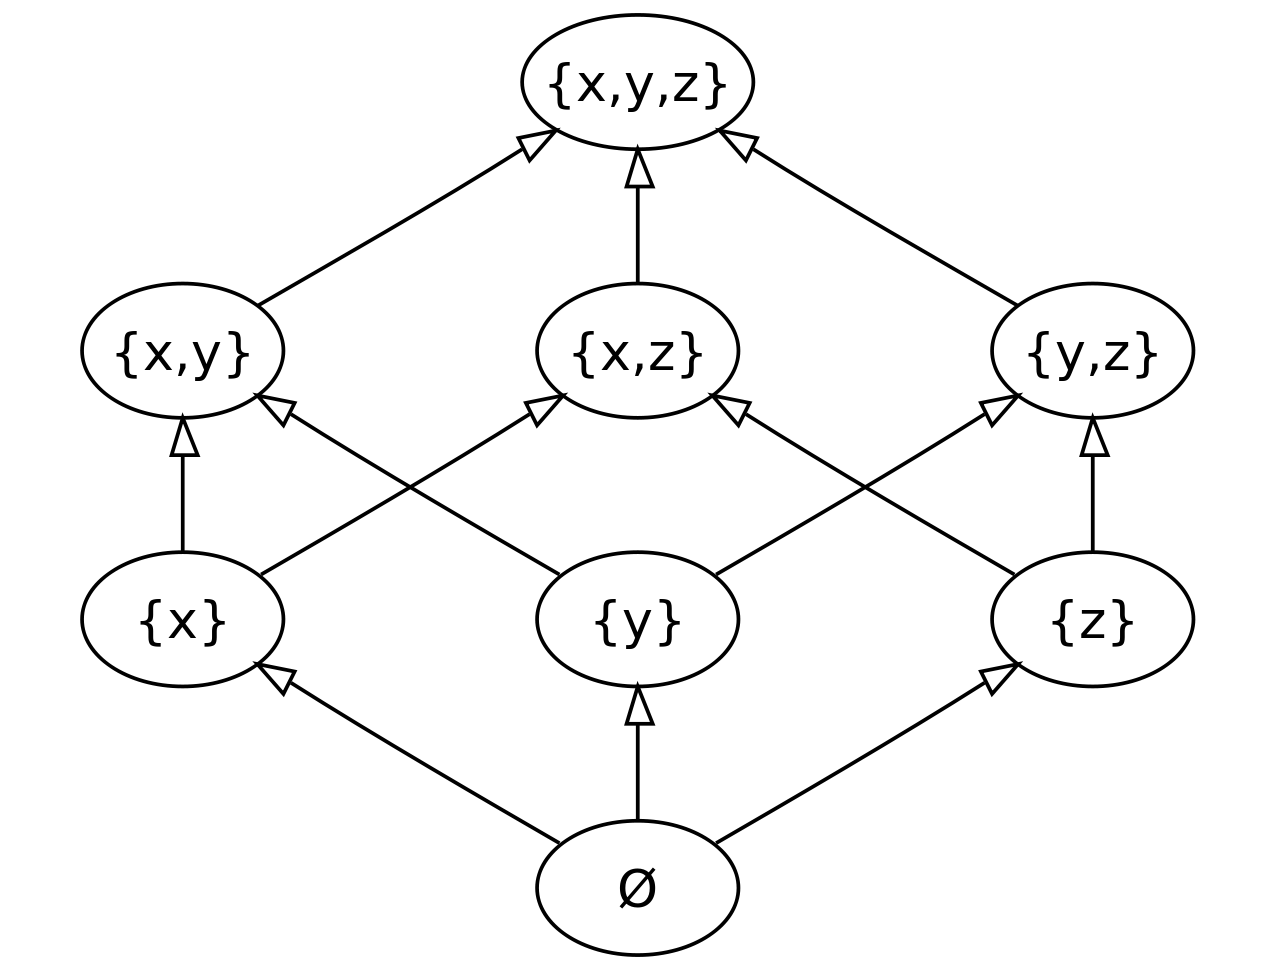
\includegraphics[width=\linewidth]{./images/hasse}
\caption{Annotation of a digitized map}
\label{figure:hasse}
\end{figure*}

A Hasse diagram can also visual concept lattices. The research group already computed a concept lattice and tries to visual it with Hasse diagrams. The result is shown in Figure~\ref{figure:firstVisualizaion}. They are not satisfied  with it because it is hard to see anything on it. The labels are overlapping and make it nearly impossible to read them. The huge number of edges make it hard to see anything.  \\

\begin{figure*}[!ht]
	\centering
	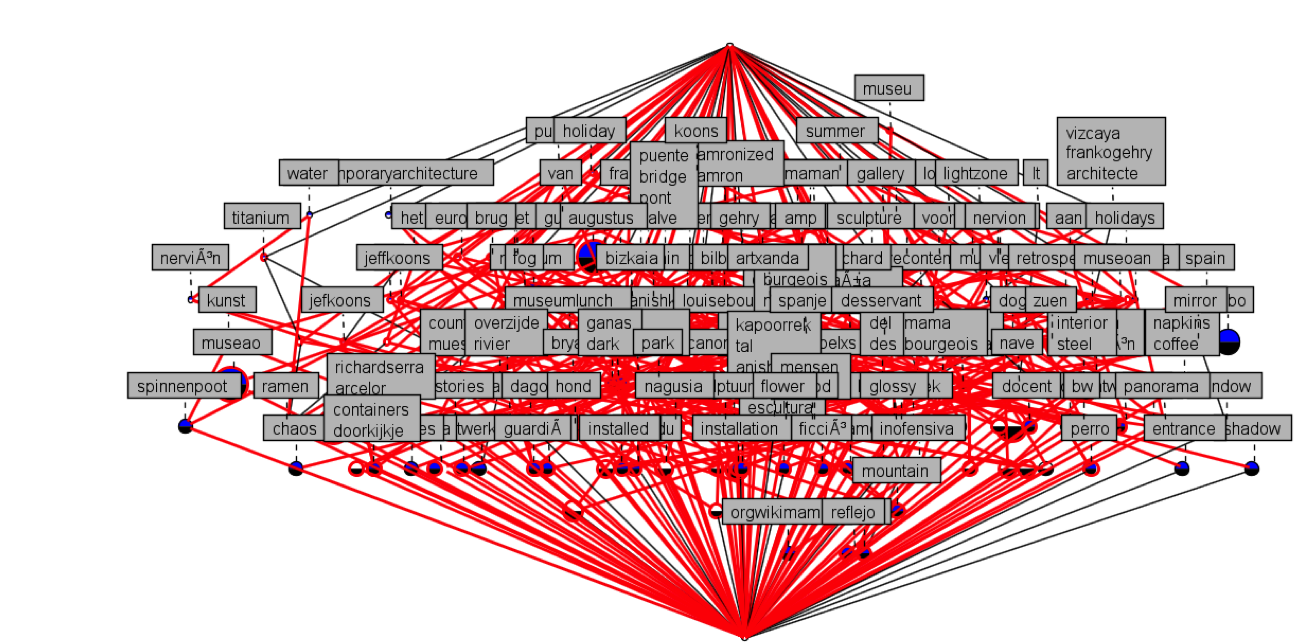
\includegraphics[width=\linewidth]{./images/firstVisualization}
\caption{First visualization of digital humanist data with traditional \acrshort{fca} software}
\label{figure:firstVisualizaion}
\end{figure*}

It is my task to create an interactive visualization of their concept lattice. The visualization should convey the information of a concept lattice even if the concept lattice is large. \\

 The remainder of this thesis is structured as follows: The background of Formal Concept Analysis and Interface Design are presented in Section~\ref{Background}. The discussion of related work takes place in Section~\ref{Related Work}. Inferring from the related work, I will present my work including idea and implementation in Section~\ref{Fancy 1.0}. In Section~\ref{Evaluation}, the evaluation takes place. Built upon the results of the evaluation, a new version is presented in Section~\ref{Fancy 2.0}. Eventually concluding in Section~\ref{Conclusions}.
 
\chapter{Background}
\label{Background}

This sections gives background knowledge before we can discuss related work in the following section. First, it gives an introduction into formal concept analysis taken from the work from Ganter and Wille \cite{Ganter2012}. Second, it introduces some user interface design principles.

\section{Formal Concept Analysis}
\label{Formal Concept Analysis}

\acrlong{fca} (\acrshort{fca}) is a mathematically well-founded technique to analyze data. \acrshort{fca} creates relationships among objects specified by attributes. It derives from old philosophical ideas and was formalized by Rudolf Wille. First, we describe the formal definitions and explain them with examples. Second, we give examples for the use of \acrshort{fca} in \acrlong{ir} (\acrshort{ir}).

\subsection{Definition}

\acrshort{fca} \cite{Ganter2012} is constructed on a formal context. A \textit{formal context} is defined as a tripple $K = (G, M, I)$ where $G$ is a set of objects\footnote{$G$ derives from German "Gegenstände".}, $M$ is a set of attributes\footnote{$M$ derives from German "Merkmale".} and $I$ is a binary relation $I \subseteq G \times M$. $I$ specifies whether an object has an attribute or not\footnote{$I$ derives from German "Inzidenzrelation".}. Table~\ref{table:example} illustrates an example from David Eppstein \cite{fcaexample} where $G$ comprises the integers from 1 to 10 and $M$ comprises the attributes composite, even, odd, prime and square. \\


\begin{table}[h]
\caption{Formal context, integers 1 to 10 as objects with attributes}
\label{table:example}
\centering

\def\arraystretch{1.2}% 
\begin{tabular}{ | c | c c c c c |}
\hline
  & composite & even & odd & prime & square\\
\hline

1 & & & $\times$ & &$\times$\\ 
2 & & $\times$ & & $\times$ &\\
3 & & & $\times$ & $\times$ &\\ 
4 & $\times$ & $\times$ & & & $\times$\\
5 & & & $\times$ & $\times$ &\\
6 & $\times$ & $\times$ & & &\\
7 & & & $\times$ & $\times$ &\\ 
8 & $\times$ & $\times$ & & &\\
9 & $\times$ & & $\times$ & & $\times$\\
10 & $\times$ & $\times$ & & &\\ \hline


\end{tabular}
\end{table}

Let the operator $'$ for $A \subseteq G$ be defined as following:
\begin{align*}
	A' = \{ m \subseteq M\; |\;  I(g, m)\;   \forall g \in A\}
\end{align*}

$A'$ is the set of those attributes that are present in all objects from given $A$. \\

Let the operator $'$ for $B \subseteq M$ be defined as following:
\begin{align*}
	B' = \{ g \subseteq G\; |\;  I(g, m)\;   \forall m \in B\}
\end{align*}

$B'$ is the set of objects that have at least the attributes given in $B$. \\

If for $A \subseteq G$ such that $A = A''$, then $A$ is called \textit{closed}. The same is true for $B \subseteq M$ and $B = B''$. \\

For example, let a set of objects be defined as $A_1 = \{1,4\} \subseteq G$. This results into: $A_1' = \{square\}$ and $A_1'' = \{1,4,9\}$. $A_1$ is not closed but $A_2 = \{1,4,9\} \subseteq G$ is called closed because $A_2 = A_2''$. \\   

A \textit{formal concept} is a pair of $(A, B)$ where $A \subseteq G$ and $B \subseteq M$ and $A = B' \wedge B = A' $. Informally, all objects in $A$ share exactly the same attributes in $B$. $A$ is a set of objects called the \textit{extent} of a formal concept. $B$ is a set of attributes called the \textit{intent} of a formal concept. The extent and the intent of all formal concepts are always closed.\\

From the example in Table~\ref{table:example}, we can derive several formal concepts. Three randomly chosen concepts are shown in Table~\ref{table:exampleConcepts}. \\

\begin{table}[h]
\caption{Three formal concepts from the formal context in Table~\ref{table:example}}
\label{table:exampleConcepts}
\centering

\def\arraystretch{1.2}% 
\begin{tabular}{ c c c }
\hline
 Concept & Extent & Intent \\
\hline

$C_1$ & \{4,6,8,10\} & \{composite, even\} \\
$C_2$ & \{2,4,6,8,10\} & \{even\} \\
$C_3$ & \{9\} & \{composite, odd, square\} \\

\hline
\end{tabular}
\end{table}

It is always possible to define an order relation on the formal concepts. Let us introduce the relation $\le$ as follows:
\begin{align*} (A_i,B_i) \le (A_j, B_j) \Longleftrightarrow	A_i \subseteq A_j
\end{align*}

With the help of $\le$, we  can derive relationships from the concepts in Table~\ref{table:exampleConcepts}. We see that $C_1 \le C_2$. This means that $C_1$ is more specific than $C_2$ and $C_2$ is more general than $C_1$. We can also see that $C_3$ is unrelated to $C_1$, and that $C_3$ is unrelated to $C_2$. \\

A formal context with $\le$ is called a \textit{concept lattice} of the context. It can be shown, that for two formal concepts $C_i$ and $C_j$, there always exists a formal concept $C_x$ such that $C_i \le C_x \wedge C_j \le C_x$. That means that there is always a formal concept wich is 'above' in the hierarchy and also related to the two formal concepts $C_i$ and $C_j$. A formal definition would exceed this section. The interested reader is advices to read "The Basic Theorem on Concept Lattices" as described by Carpineto and Romano on page 13 in their work \cite{carpineto2004concept}.\\

In the next section we will take a look at the static visualization of concept lattices.

\subsection{Static Visualization}

It is often said that a picture is worth a thousand words. To convey the information of a concept lattice, it can be visually represented in a \textit{Hasse diagram} \cite{Ganter2012}. Figure~\ref{figure:example} shows the Hasse diagram of the concept lattice derived from the formal context described in Table~\ref{table:example}. \\

\begin{figure*}[!ht]
	\centering
	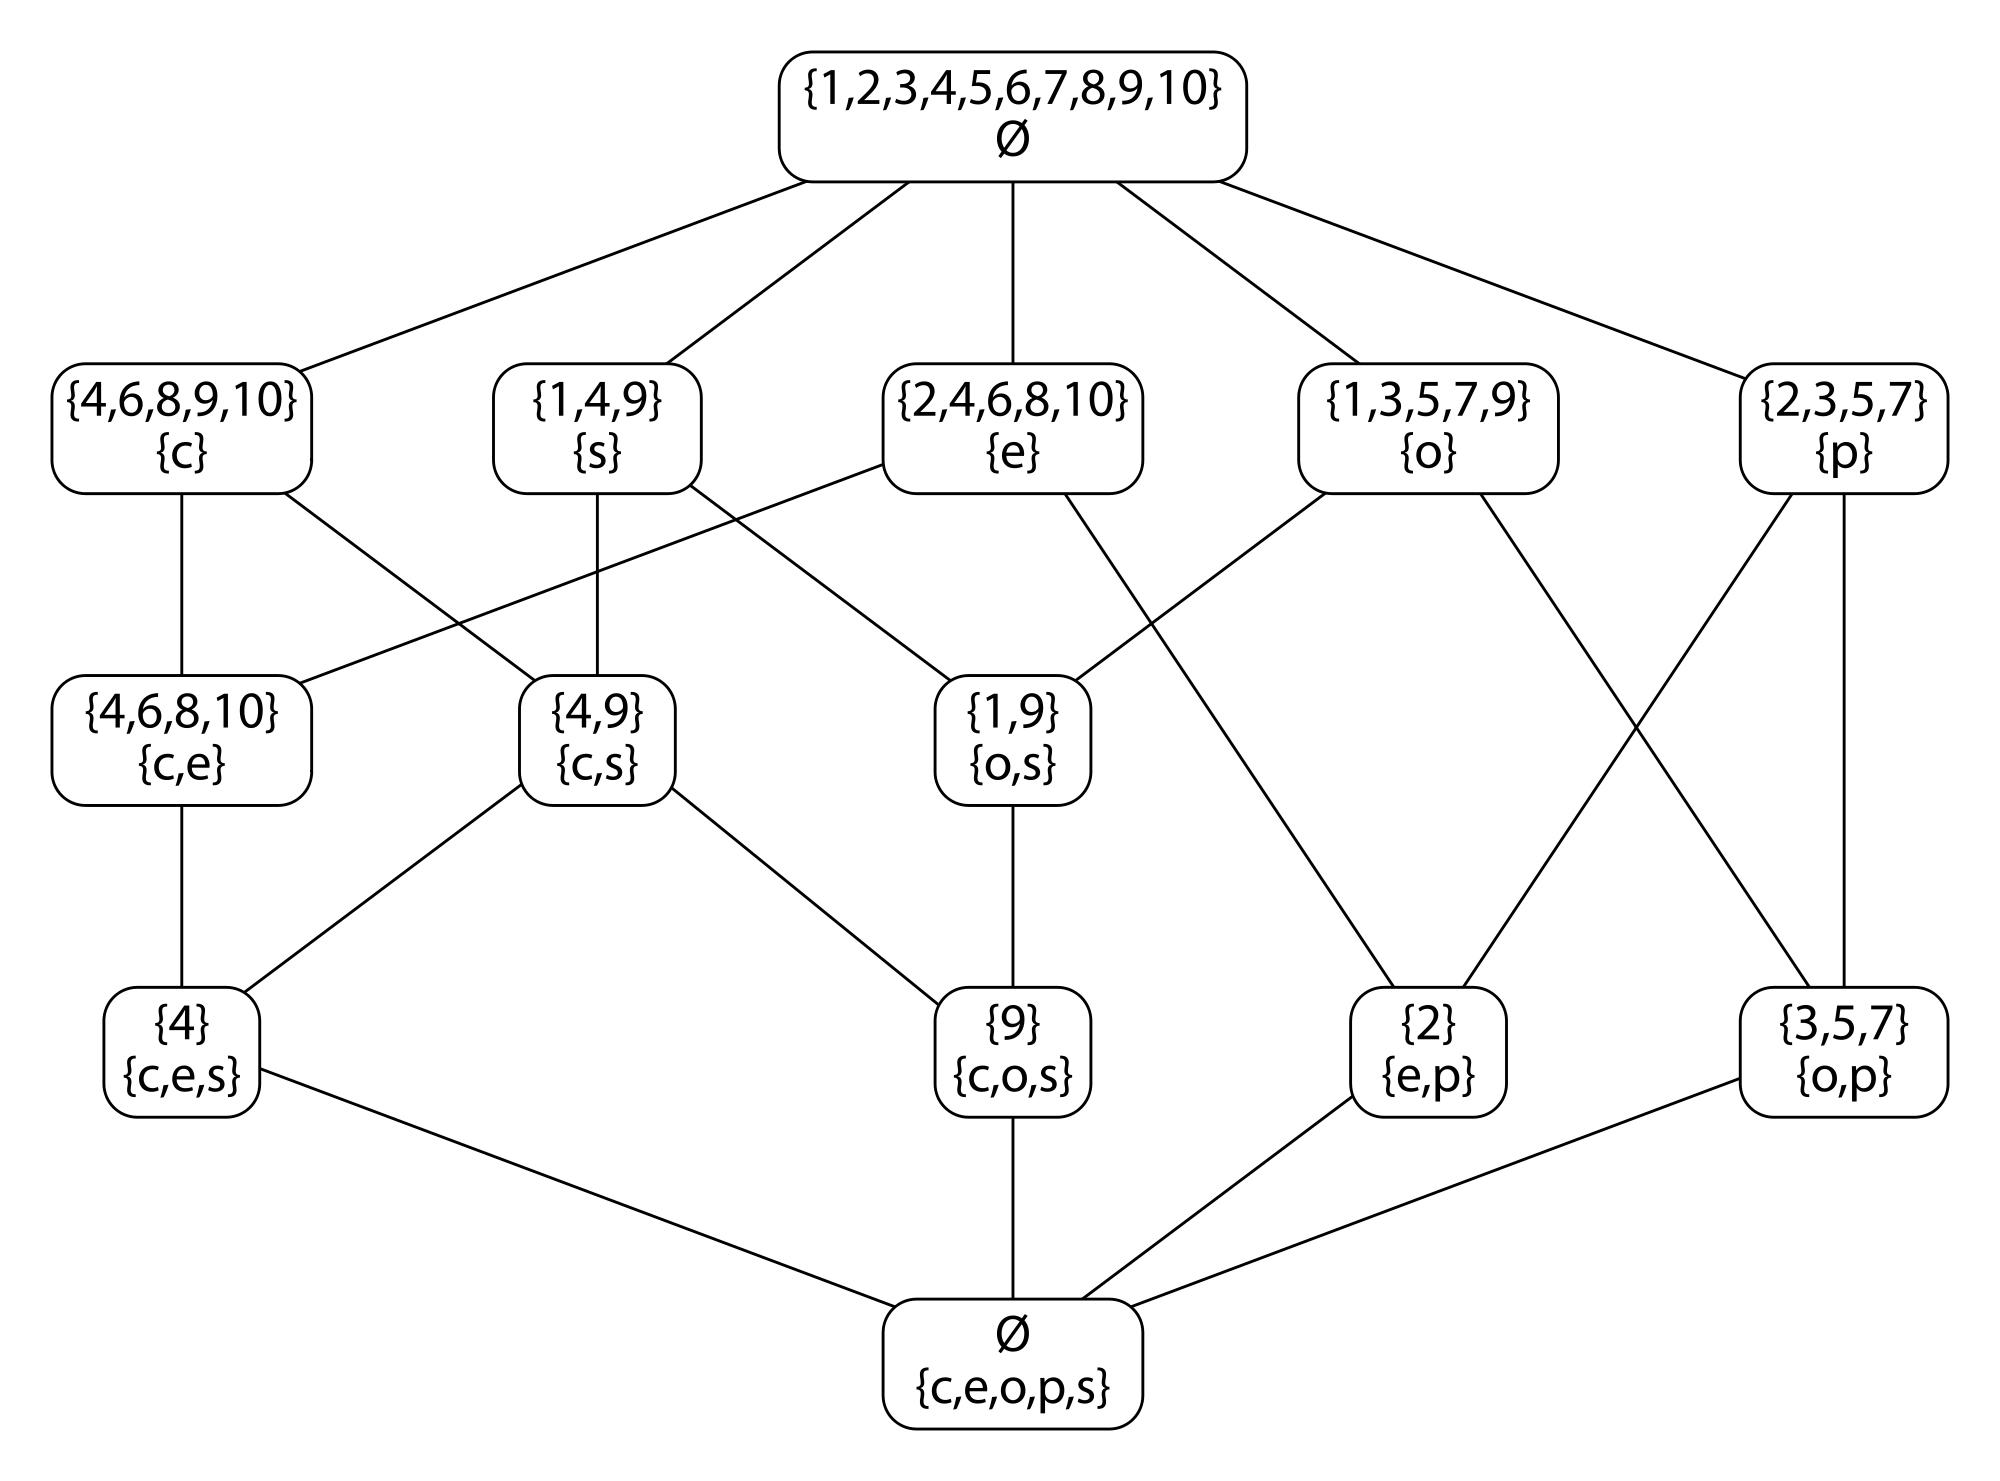
\includegraphics[width=\linewidth]{./images/fcaExample}
\caption{Hasse diagram, with the integers 1 to 10 as objects and attributes square (s), prime (p), composite (c), even (e), and odd (o). Source: Eppstein \cite{fcaexample}}
\label{figure:example}
\end{figure*}

A Hasse diagram is a graph where the vertices represent formal concepts and edges represent the relation $\le$ among the formal concepts. An edge between formal concepts $C_i$ and $C_j$ is drawn, when $C_i \le C_j$ and there does not exist a formal concept $C_x$ such as $C_i \le C_x \le C_j$. To increase the readability, the nodes are ordered in layers. The concepts in top are more general, the concepts in the bottom are the more specific ones.\\

There are two special concepts: \textit{supremum} and \textit{infimum}. The supremum is vertex node in the top and the attributes in its intent are those which are present in all objects. In most cases its intent is empty. The infimum is the vertex in the bottom and the objects in its extent are those which have all attributes. In most cases its extent is empty.\\

After this general introduction, we will describe in the next section how we can apply \acrshort{fca} to \acrshort{ir}.

\subsection{Application of \acrshort{fca} in \acrshort{ir}}
\label{section:fcair}

Up to now, we only showed primitive examples to illustrate the basics of \acrshort{fca}. So where was it applied? According to Poelmans et al. \acrshort{fca} has been "applied in many disciplines such as software engineering, knowledge discovery and \acrshort{ir}" \cite{Poelmans2013}. They did two comprehensive surveys on the application of \acrshort{fca} \cite{Poelmans2013, Poelmans2013b}. \\

In the case of IR on a document collection, the objects are the documents. These documents are described by index terms. These index terms are the attributes of the objects. In Table~\ref{table:fcair} are documents described by index terms take from Godin et al. \cite{Godin1993}. The concept lattice is visualized in Figure~\ref{figure:fcair}.

\begin{table}[h]
\caption{Documents described by Index Terms, from Godin et al. \cite{Godin1993}}
\label{table:fcair}
\centering

\def\arraystretch{1.2}% 
\begin{tabular}{ | l | l | }
\hline
 Document & Index Terms \\
\hline

1 & \{animal, bear, canada, child, cow-boy, dream, fantasy,\\
  & immigration, indian, magic\} \\
2 & \{animal, cat, child, fantasy, magic, tale\} \\
3 & \{animal, child, dog, fair, fantasy, love, parade\} \\
4 & \{child, fantasy, friendship, game, rope\} \\
5 & \{creativity, child, fantasy, game, music, sound\} \\
6 & \{animal, child, dream, fair, fantasy, friendship, octupus\} \\

\hline
\end{tabular}
\end{table}

\begin{figure*}[!ht]
	\centering
	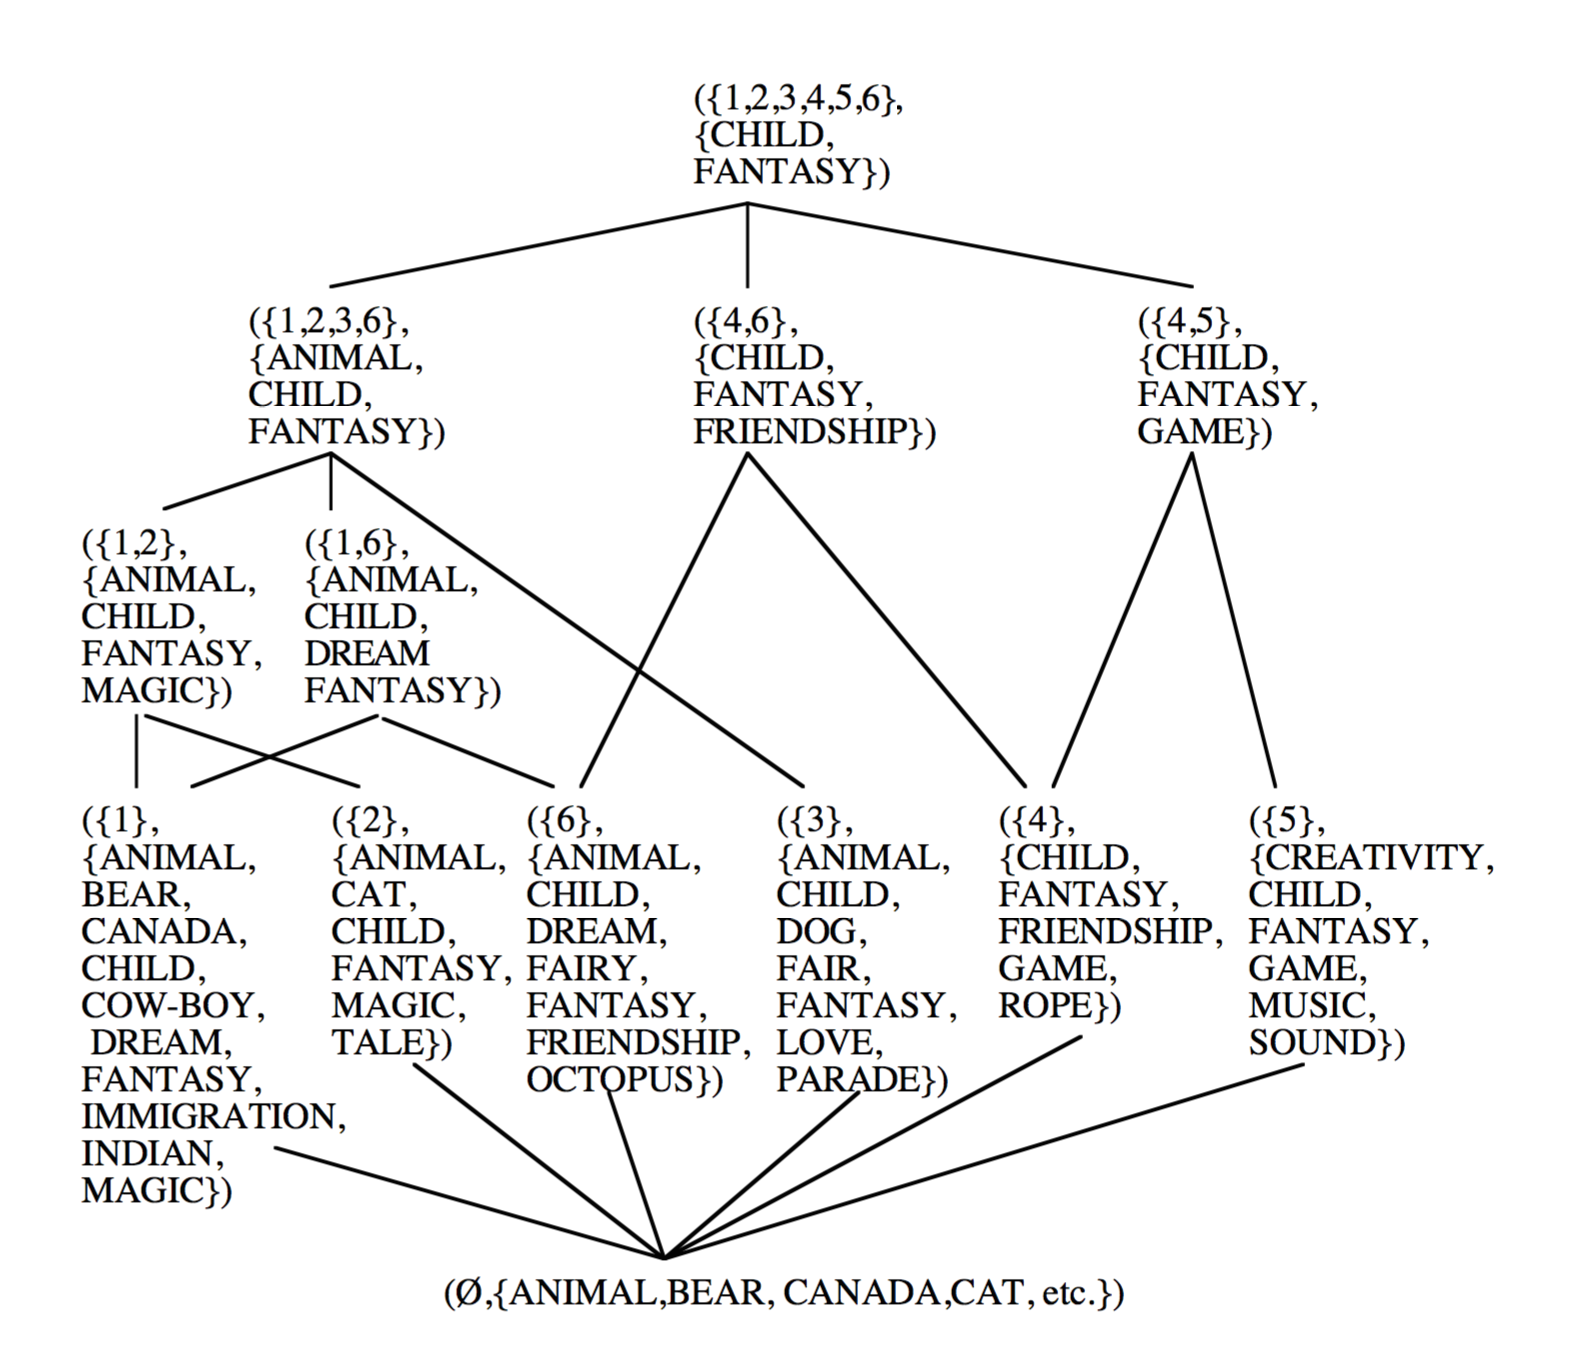
\includegraphics[width=\linewidth]{./images/fcair}
\caption{Hasse diagram from concept lattice derived from \ref{table:fcair}. Source: Godin et al. \cite{Godin1993}}
\label{figure:fcair}
\end{figure*}

Carpineto and Romano \cite{Carpineto2005} describe that a concept can be seen as a query (intent) with a set of retrieved documents (extent) and that neighboring concepts can be seen as minimal query changes. When the user queries a FCA-based system, the intents of the formal concepts are checked for a match (or a partial match if there is no match in the first place). So for instance with the query "child fantasy friendship" the document 4 and 6 wold be retrieved. You find the concept in the middle of the Hasse diagram. The neighboring concepts are connected with an edge. \\


Sacco and Tzitzikas \cite{Sacco2009} describe two information access modes: \textit{focalized search} and\textit{exploratory search}. In focalized search, the user is interested to find relevant information to a given query. In opposite to exploratory, where the user explores relationships among items in a data collection. While FCA provides the user with the ability to do focalized search, it offers sophisticated exploratory capabilities. When the user queries the system (as described above), not only the documents of the formal concepts are retrieved, but she can also see the position in the lattice. Is the concept in the upper half and thereby more general? Or is it in the bottom half and thereby more specific? What are the related formal concepts? How do they differ? Would there be a lot more documents if I would remove a term from the query? All this questions can be answered and because the whole lattice is already computed, relatively fast. Without going into detail, a major problem of FCA is the time-consuming creation of a lattice. But this focus of this thesis is the visualization of concept lattices and not the creation of concept lattices. This section should give a slight introduction and the interested reader is advised to study the work from Carpineto and Romano \cite{carpineto2004concept} for a detailed investigation. \\

This work develops an interface for one specific datasets. That is why it is important the lattice structure of this dataset how it was created. The next section described the dataset.

\subsection{The Data}
In the following, I will described how the research group created the data on which this thesis is based. \\

The research group asked human scholars for a list of 100 interested words. This list is the dictionary. The index terms of a documents specify if this index terms is present in the document. They were 7492 documents with 100 possible attributes, the index terms. They result into a concept lattice with 131379 formal concepts.\\

Because this thesis focuses on the user interface, let us review user interface design principles before we discussed related work in Section~\ref{Related Work}.

\section{Interface Design}
\label{id}

The user interface is responsible for the interaction with users. The interaction of humans with computers has its own research area, \acrlong{hci} (\acrshort{hci}), and one of its pioneers is Ben Shneiderman. In the following, two principles from him are presented: The "Eight Golden Rules of Interface Design" \cite{Shneiderman2010} and the "Visual Information Seeking Mantra" \cite{Shneiderman1996}.

\subsection{Eight Golden Rules of Interface Design}
\label{Golden}

These rules \cite{Shneiderman2010} are genreal advices for user interface designers which should apply to all interfaces. The rules are named and explained with my own remarks. \\

\begin{itemize}
	\item Strive for consistency: Use similar actions in similar situations. Use identical terminology, colors, fonts etc. throughout the system.	
	\item Cater to universal usability: Design for the needs of a diverse user group (skill level, age, gender and others)
	\item Offer informative feedback: Give system feedback for every action.
	\item Design dialogs to yield closure: Sequences of actions should be grouped. Give feedback on completion of a group.
	\item Prevent errors: Design the system that the user cannot even do errors in the first place. But if she does some, offer instructions how to recover.
	\item Permit easy reversal of actions: Actions should be undone. This gives the user confidence to explore the system.
	\item Support internal locus of control: The user should think that she is in charge of control.
	\item Reduce short-term memory load: Reduce the number of things the user has to keep in mind while using the system.
\end{itemize}

There exits alternative principles for instance: Donald Norman's Design Principles \cite{Norman2013} or Jakob Nielsen's "10 Usability Heuristics for User Interface Design" \cite{Nielsen1995}. They are very similar and only differ points not worth mentioning. \\

These principles can be applied to all user interfaces. In the next section, design principles will be presented which are more related to this work.

\subsection{Visual Information Seeking Mantra}

The visual information seeking mantra (the Mantra) was introduced by Ben Shneiderman \cite{Shneiderman1996} and is based on his experience with past projects. Albeit the Mantra was intended to be a "descriptive and explanatory" \cite{Card1999}, "in effect, the Mantra has become a prescriptive principle for many information visualization designers" write Craft and Cairns \cite{Craft2005}. \\

The Mantra describes design principles for interfaces when user view collection of items. This items are described by multiple attributes. The starting principles are: overview first, zoom and filter, and then details on demand. These four principles will be explained below and extended by three other principles.
\begin{itemize}
	\item Overview: Gain an overview of the entire collection.
	\item Zoom: Zoom in on items of interest.
	\item Filter: Filter out uninteresting items.
	\item Details-on-demand: Select an item or group and get details when needed.
	\item Relate: View relationships among items.
	\item History: Keep a history of actions to support undo, replay, and progressive refinement.
	\item Extract: Allow extraction of sub-collections and of the query parameters.
\end{itemize}

Some tasks need more explanation.

\subsubsection{Zoom and Filter}

This task are responsible for reducing the complexity of the data collection. 'Zoom' means that the user focuses on items she wants to see. 'Filter' means that she can hide items which are not interesting for her.

\subsubsection{History}

It is important to give the user the possibility to easily recover from mistakes or loss of interest. In addition, "it is rare that a single user action produces the desired outcome. Information exploration is inherently a process with many steps, so keeping the history of actions and allowing users to retrace their steps is important." writes Shneiderman \cite{Shneiderman1996}.

\subsubsection{Extract}

Once interesting objects are found, the user should have the possibility to extract them from the system. Shneiderman describes printing, emailing or saving the item to the disk as 'extraction'.

\subsection{Final Remarks}

The presented ideas are based mostly on the experience of one person: Ben Shneiderman. The huge number of citations show that his work is influential but Craft and Cairns \cite{Craft2005} call for empirical justification of the Mantra. \acrshort{hci} is a young research area and they will come better and more polished guidelines the future. Until then, the work from Ben Shneiderman seems to be valid starting point. \\

Those principles are up to interpretation and adaption. Every system is different and has its different needs. For this reason, let us review what other people did and how they designed their interface for \acrshort{fca}-based systems.

\chapter{Related Work}
\label{Related Work}

After introducing formal concept analysis in Section~\ref{Formal Concept Analysis}, let us review and discuss related work. In the first three sections, we go over different \acrshort{fca}-based approaches. Eventually, we evaluate one \acrshort{fca}-based approach in detail: The Virtual Museum of the Pacific. In Section~\ref{dyafs}, a non-\acrshort{fca} based approach is shown which is related to \acrshort{fca}: \acrshort{dt} and Faceted Search. \\

\section{Full Hasse Diagrams}

The traditional, static visualization of concept lattices are Hasse diagrams as describes in Section~\ref{Formal Concept Analysis}. Eklund et al. \cite{Eklund2004} conducted user studies and proclaim that non-\acrshort{fca}-experts can read Hasse Diagrams if you fine-tune the Hasse diagram. For instance by choosing appropriate colors, using symbols and carefully positioning the vertices in layer. \\

But in the domain of \acrshort{ir} you get formal contexts with a lot of objects. Hasse diagrams scale bad for large concepts lattices. Kuznetsov et al. \cite{Kuznetsov20072}  describe this resulting visualization: "Representing concept lattices constructed from large contexts often results in heavy, complex diagrams that can be impractical to handle and, eventually, to make sense of." Especially the high connectivity of the graph results in enormous edge crossing. The Figure~\ref{figure:firstVisualizaion} shown in Section~\ref{Introduction} shows the first result of the research group. The visualization is useless because it is not even possible to see all the labels. In the next section we describe techniques to improve the situation.

\section{Pruned Hasse Diagrams}

The Hasse diagrams can be pruned by reducing the number of vertices. The different techniques are discussed in the next section.

\subsection{Reduce Number of Formal Concepts}

One way to reduce the number of vertices is to compute the \textit{iceberg lattices} as described by Stumme et al. \cite{Stumme2002}. They result after the application of a data mining technique "frequent item-set mining" from Agrawal et al. \cite{Agrawal1993}. Only formal concepts are selected which are considered "frequent". A formal concept is frequent if its intent, the set of attributes, is frequent. Let $B$ be the intent and $minSupport \in [0, 1]$, then $B$ is frequent if $ |B'|/|G| \geq minSupport$. This means the attribute set has to specify a high portion of objects; at least $minSupport$. This approach has some drawbacks as Kuznetsov et al. \cite{Kuznetsov20072} point out that "exotic" or "emergent" concepts that are not represented by a large number of objects can be interesting too and should not been overlooked. They propose to only select "stable" concepts \cite{Kuznetsov20072}. The intent of stable concepts does not depend much on each object of the extent. It is also possible to apply traditional cluster techniques like fuzzy K-Means clustering to \acrshort{fca} \cite{AswaniKumar2010}. \\

	While all these techniques undoubtable reduce the number of formal concepts, it is to question if the results are any helpful. In our case of \acrshort{ir}, we apply \acrshort{fca} to explore the data and get insights about the lattice structure. When pruning the nodes, you are losing many data relationships, many formal concepts and, consequently, the "power" of \acrshort{fca} as exploratory technique is significantly reduced. When we deal with large concept lattices, the number of nodes has to be very low if we want to represent them with Hasse diagrams. Nowadays, the question is not how do I visualize 16 formal concepts as in Figure~\ref{figure:example} - it is more how can I analyze 160.000 formal concepts.\\
	
	Pruning alone is not a proper way to handle large concept lattice. But it can be useful to reduce the clutter. It can be useful in combination with techniques that are presented in Section~\ref{Local View}.
	
\subsection{Nest Formal Concepts}	

Another approach are \textit{nested line diagrams} - line diagrams are another name for Hasse diagrams. For this, all attributes are partitioned into layers. For example, if you just have two layers, an attribute is either in layer one or two. For the first layer: You built up a Hasse diagram with the attributes \textit{solely} of the first layer. For each vertex in the resulting Hasse diagram, you built up a Hasse diagrams \textit{inside} the vertex. This secondary Hasse diagrams are built from the concept lattice derived from the objects in the vertex (the objects that are the extent of the formal concept). This can be done for an arbitrary number of layers. An example from Carpineto and Romano \cite{carpineto2004concept} is shown in Figure~\ref{figure:nested}. The general idea should be clear without explaining the context - if not Carpineto and Romano \cite{carpineto2004concept} describe it more in detail. \\

\begin{figure*}[!ht]
	\centering
	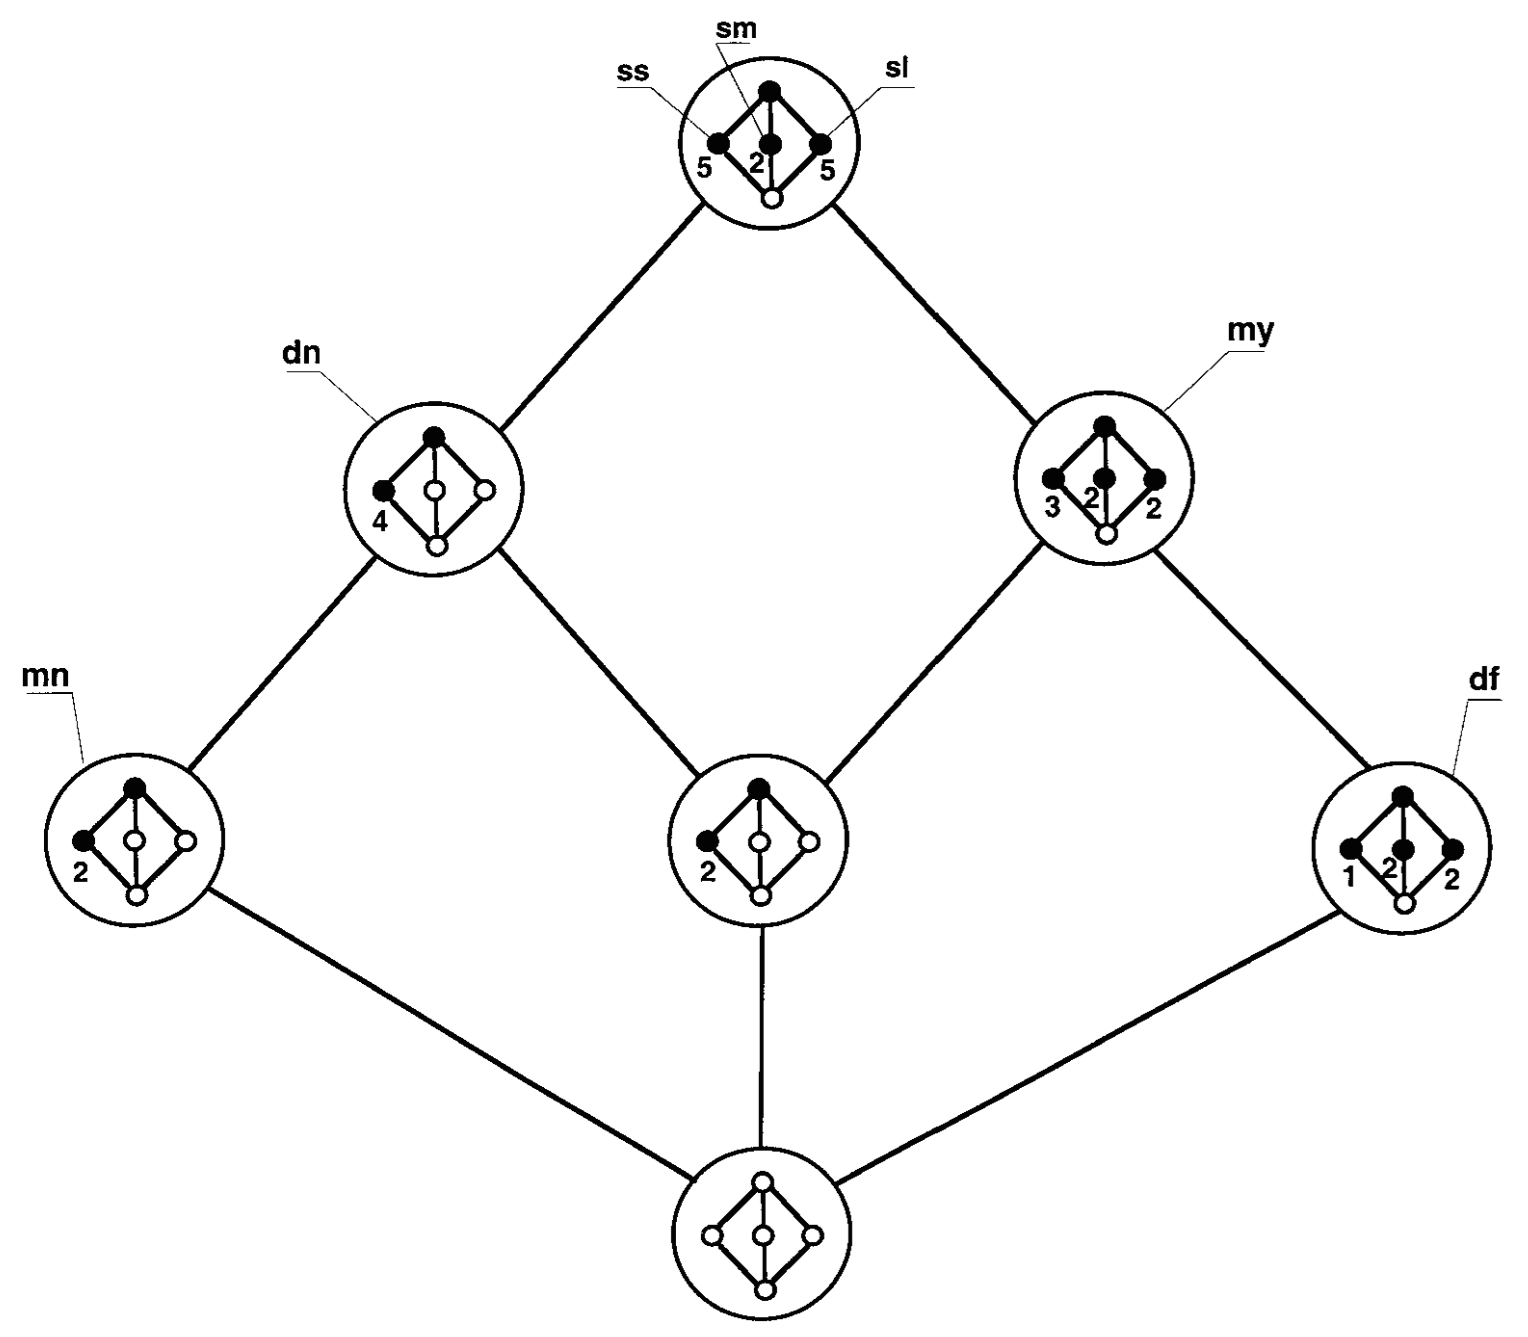
\includegraphics[width=\linewidth]{./images/nested}
\caption{Nested line diagram with two layers. Source: Carpineto and Romano \cite{carpineto2004concept}}
\label{figure:nested}
\end{figure*}
	
But how to partition the attributes? You have to select the partitions manually. The manual selection might be good idea of small concept larges but in our case it is not feasible.

\section{Local View}
\label{Local View}

Instead of showing the full Hasse diagram, the user can have a local view on the lattice. We will give an overview about the basic idea and applications before we review one real-world application in detail. \\

\subsection{Introduction}

One could argue that you just have to visualize everything and then allow to zoom on nodes. This techniques is common among network visualizations \cite{Herman2000}. But because of the high connectivity of the graph, this is not helpful to Hasse diagrams. You can see this at the tool 'FCART' presented by Neznanov and Parinov \cite{Neznanov2014}. In Figure~\ref{figure:fcart} they visualize a concept lattices comprising more than 20000 concepts. \\

\begin{figure*}[!ht]
	\centering
	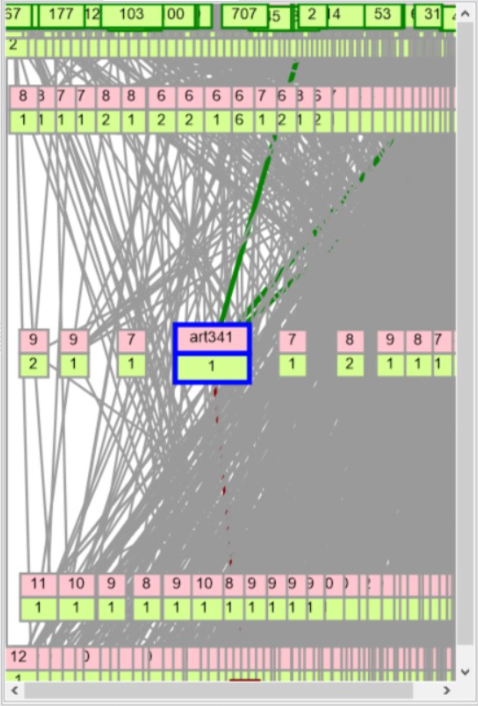
\includegraphics[width=0.5\linewidth]{./images/fcart}
\caption{FCART, Hasse diagram visualization with over 20000 formal concepts, focus on node with blue borders. Source: Neznanov and Parinov \cite{Neznanov2014}}
\label{figure:fcart}
\end{figure*}

Even though they chose a grey color for the edges, the screen is almost filled only with the grey. In addition, they labels of the nodes in the top and bottom are overlapping which makes it hard to read them. Let us review some other approaches in the next section which completely break with the Hasse diagram.

The local view on a Hasse diagram is called \textit{conceptual neighborhood} by Eklund et al. \cite{Eklund2009,Eklund2012} or \textit{hybrid navigation} by Carpineto and Romano \cite{Carpineto1996}. The basic idea is always the same: The interface is always focused on exactly \textit{one} formal concept. The user can navigate through the lattice by going up (becoming more general) or going down (becoming more special). Which means removing terms or adding terms. They also offer the possibility to query the system. In most cases, the user would start with a search and focuses on the corresponding formal concept if it exists. From there, the user can fine-tune the search. The idea originated from the \acrshort{ir} field and was first proposed by Godin et al. \cite{Godin1989}. \\

At least three ideas underly this approach. First, users tend to start with a short query and then refine their needs. Hearst \cite{Hearst2009} write  while referring to \cite{Marchionini2006,Bates1990}:
\begin{quote}
	"A commonly-observed search strategy is one in which the information seeker issues a quick, imprecise query in the hopes of getting into approximately the right part of the information space, and then doing a series of local navigation operations to get closer to the information of interest."
\end{quote}

Second, it easier for the users to choose from suggestions than to formulate a query. Aula \cite{Aula2005} writes that searching is more demanding method for locating information than browsing, as it involves several phases, such as planning and executing queries, evaluating the results, and refining the queries, whereas browsing only requires the user to recognize promising-looking links. \\

Third, after the initial search, the neighboring concepts are basically suggestions to the users. This prevents them from getting empty results. This is related to the design principle: "Prevent errors" presented in Section~\ref{Golden}. Zero results are not really errors, but they can be seen as a failure in a search process.\\

Godin et al. \cite{Godin1993} evaluated their \acrshort{fca}-based approach in comparison to boolean retrieval and hierarchical retrieval and proclaim that their experiment suggests that retrieval using a concept lattice may be an attractive alternative since it combines a good performance for subject searching along with browsing potential."

\subsection{Applications}
Carpineto and Romano picked up the idea from Godin et al. and developed a \acrshort{fca} search engines ULYSSES \cite{Carpineto1995,Carpineto1996}. The user can fine-tune what neighboring vertices are displayed by bounding the information seeking space. They are not only showing directly adjacent vertices but also vertices that do not exceed a given distance. It is also possible to restrict the space to vertices which are above, below, left or right of the focus. The system is shown in Figure~\ref{figure:ulysses}. \\

\begin{figure*}[!ht]
	\centering
	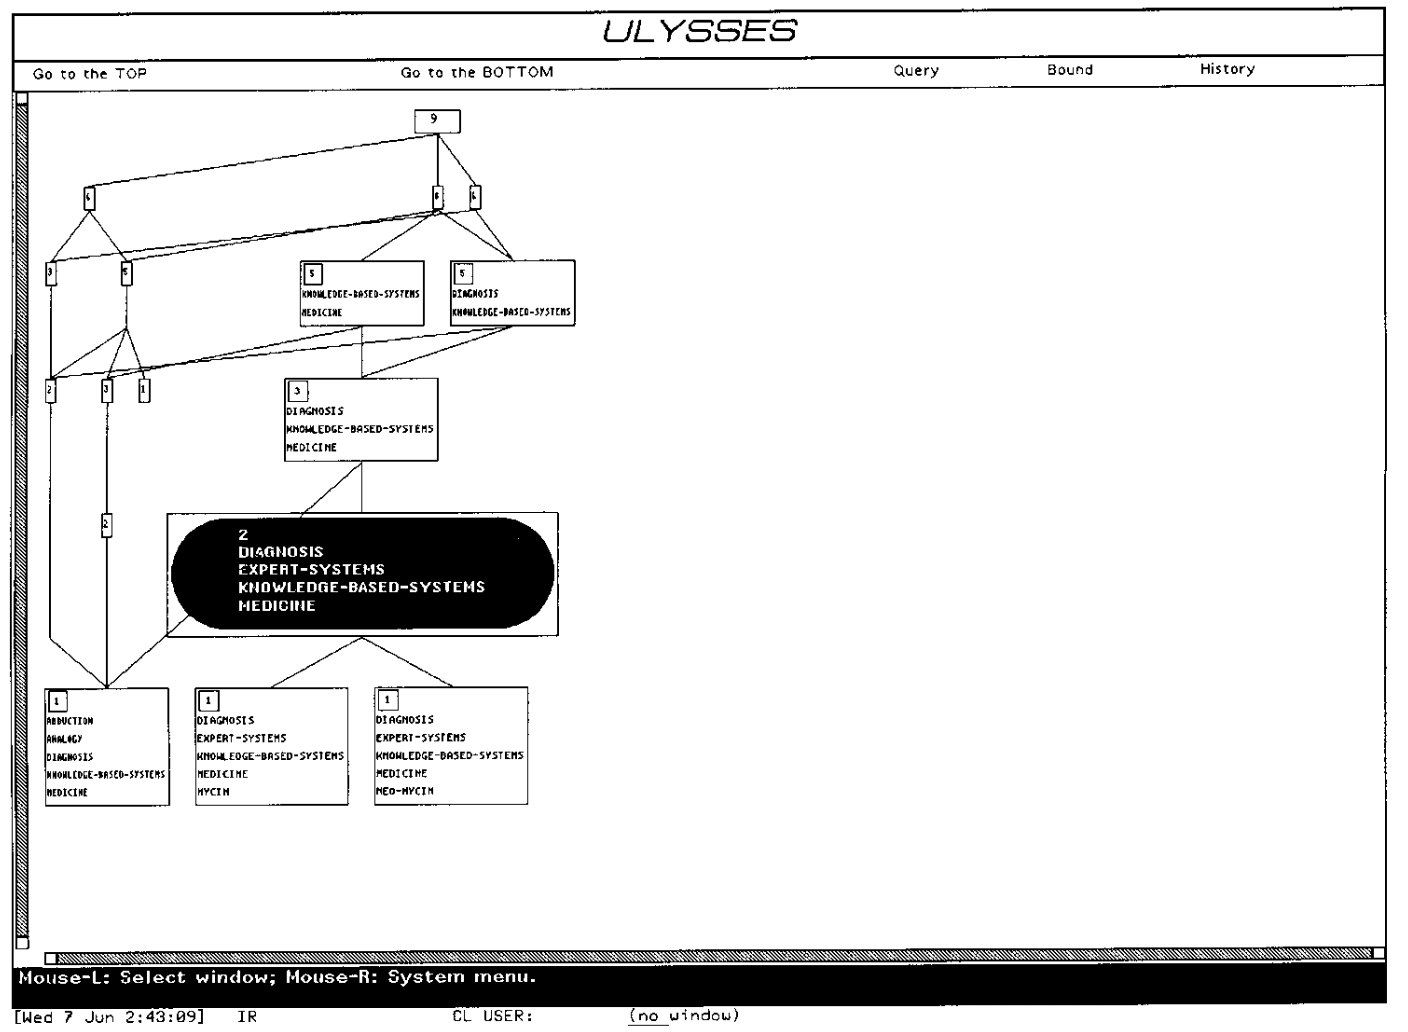
\includegraphics[width=\linewidth]{images/ulysses}
\caption{ULYSSES with focus on the black node. Source: Bach \cite{Bach2010} }
\label{figure:ulysses}
\end{figure*}

\begin{figure*}[!ht]
	\centering
	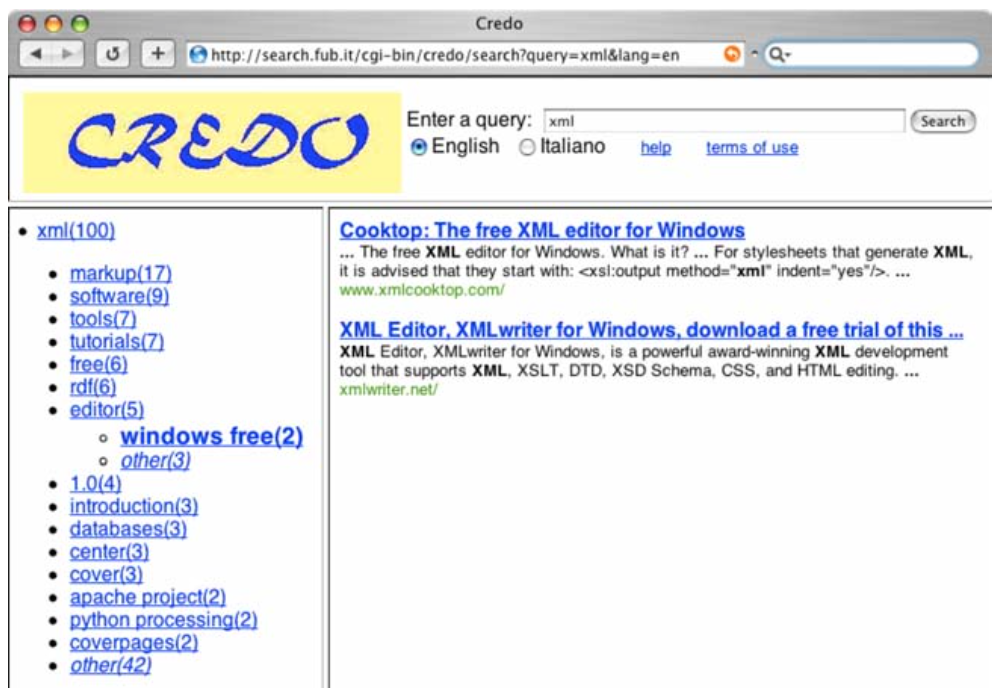
\includegraphics[width=\linewidth]{images/credo}
\caption{Screenshot of CREDO, after query 'xml' and browsing after 'editor(5)' and 'windows free(2)'. Source: Carpineto and Romano \cite{Carpineto2004} }
\label{figure:credo}
\end{figure*}

In their work, CREDO \cite{Carpineto2004}, Carpineto and Romano followed the look of ordinary search engines. The presentation of the concept lattice is not oriented at the Hasse Diagram. It looks more like a folder structure. It is shown in \ref{figure:credo}. Work that is similar comes from Koester \cite{Koester2006}, Dau et al. \cite{Dau2008}, Nauer and Yannik \cite{Nauer2009} and Cigarran et al. \cite{Cigarran2004}. In all these cases, \acrshort{fca} is applied in slightly different manner. The search is done with ordinary search engines in the background (e.g. Yahoo!) and the concept lattice is built from the results of the search. So for every new search, there is a new concept lattice. This is different from our approach, where there is just one static concept lattice. \\

Let us now review work of \acrshort{fca} on document collections. Eklund et al. applied \acrshort{fca} to email organization \cite{Eklund2004}, image browsing \cite{Ducrou2006,Ducrou2008} and a later work is the 'Virtual Museum of the Pacific' \cite{Eklund2009,Eklund2012}. We will focus on the museum because it does exactly what we are trying to do: Visualize a concept lattice built from image metadata. Furthermore it is a rare example of \acrshort{fca} outside of the academic community. It also runs in the browser and it was built in 2009 - so it is fairly recent. In addition, they conducted a usability study with museum experts and non-experts \cite{Eklund2012}.

\subsection{Virtual Museum of the Pacific}
\label{Museum}
 
The museum was created to give user the possibility to browse images of museum objects. It is available on the web\footnote{\url{http://epoc.cs.uow.edu.au/vmp/} - Credentials are required. Use username: filter and password: 45755} and it is advised to take a look at it before continue reading. \\

\begin{figure*}[!ht]
	\centering
	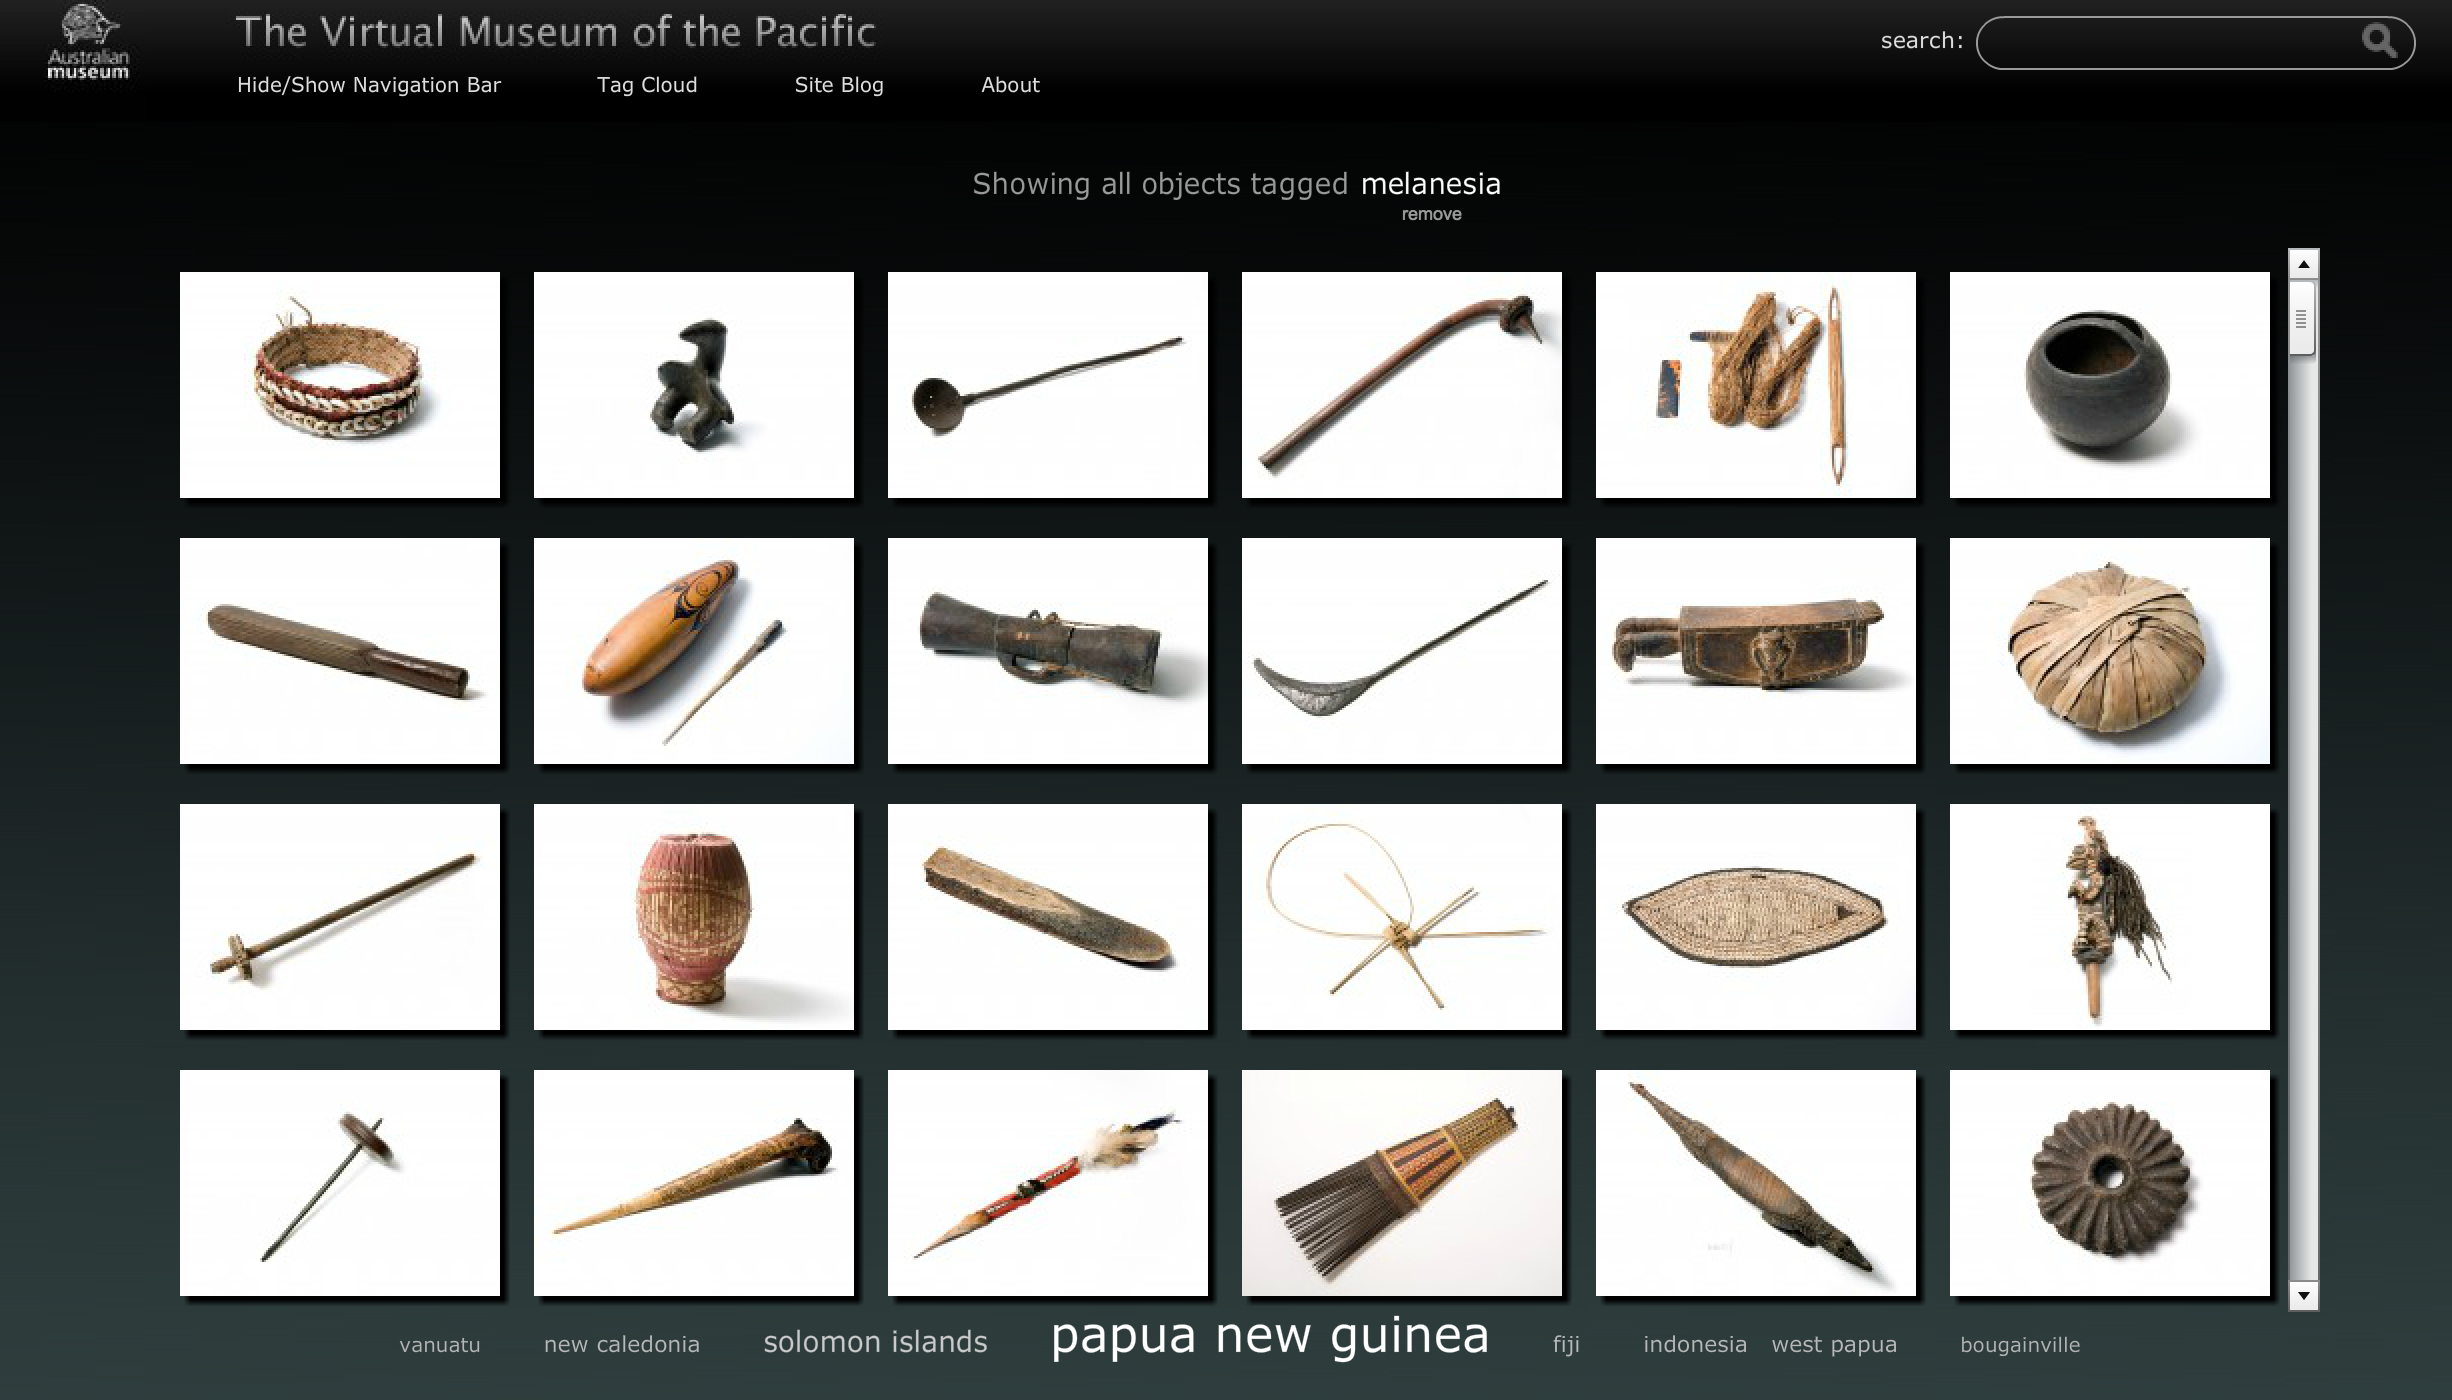
\includegraphics[width=\linewidth]{images/pacific}
\caption{The Virtual Museum of the Pacific, focus on concept 'melanesia'}
\label{figure:pacific}
\end{figure*}

After the login, the user can either search on the collection or get an overview over the collection by clicking "tag cloud" or "browse perspective". The interface sets the objects, the images, in the focus of the interface. This is, in my opinion, a good decision. The user is probably more interested in the objects than in the concept lattice. The lattice is just an artificial structure that was built around the objects. \\
 
 Above the objects is the intent of the focused formal concept. It is possible to remove terms from the current selection to generalize (go up in the lattice). Below the objects are terms suggested to specify the information needs (go down in the lattice). The view changes when the users decide to add or remove terms. The sidebar categorizes the attributes into topics. It looks like they have created a taxonomy for their attributes. This allows the users to filter out interesting terms. But the manual selection is time-intensive and it does not scale very well. It is also to question if FCA should be applied to datasets with a taxonomy. More information will follow in section~\ref{dyafs}. To get details on demand, you have to click on an item. From there you can also find related items. This views offers a good view.\\
 
 Now to the problems. It is possible to search but this search is very rudimentary. They should have stick to well-proven user search interface principles as described by Hearst \cite{Hearst2009}. The biggest problem is the missing "home" or "reset" button and the absence of any form of history. As Shneiderman \cite{Shneiderman1996} point out "Information exploration is inherently a process with many steps, so keeping the history of actions and allowing users to retrace their steps is important." We saw in Section~\ref{section:fcair} that \acrshort{fca} can bee seen as a exploratory technique. Not implementing \textit{any} possibility to backtrack is a huge problem. You can see in the evaluation that users were confused. Eklund et al. write \cite{Eklund2012}:
 \begin{quote}
 Users also had difficulty understanding the notion of conceptual navigation as a way of navigating an information space, rather than a fixed hierarchy with a well defined `home' state. [..] Many users felt `lost' within [the \acrshort{fca}-based] style of navigation. A recommendation was put forward so that users could at least back track through the navigation sequences (in the form of a `Back' button) or that users could easily go back to a `home' or `reset' state.
 \end{quote}
  In my opinion, they are not addressing these problems - even thought the navigation is \textit{the} problem with \acrshort{fca}. It feels like that they are blaming the problems on the unfamiliarity of the users when they write \cite{Eklund2012}: "there were a number of common issues, mostly relating to the unfamiliarity of the interface". This is a weak argument because users are always unfamiliar with new interfaces. But after all, this evaluation gave valuable insight into the perception of users with a local view navigation.
  
\subsection{Conclusion}

The Virtual Museum of the Pacific is one of the view examples of \acrshort{fca} that breaches out of traditional static visualizations. They idea to show only the directly related formal concepts is promising because this scales better than Hasse diagrams. My idea is based upon the work from the museum but addresses critical problems: the missing orientation, the missing history and rudimentary search implementation. The idea is described in section~\ref{Fancy 1.0}. Before that, let us review a related non-\acrshort{fca}-based technique, but feel free to skip it. \\

\section{Faceted Search}
\label{dyafs}

This section should only give a small overview about this technique. Completely introducing it is beyond the scope of the thesis. Excessive information can be found in the work from Sacco and Tzitzikas \cite{Sacco2009}. To keep things short, this technique is explained with an example. Figure~\ref{figure:flamenco} shows a screenshot of Flamenco as described by Yee et al. \cite{Yee2003}. \\

\begin{figure*}[!ht]
	\centering
	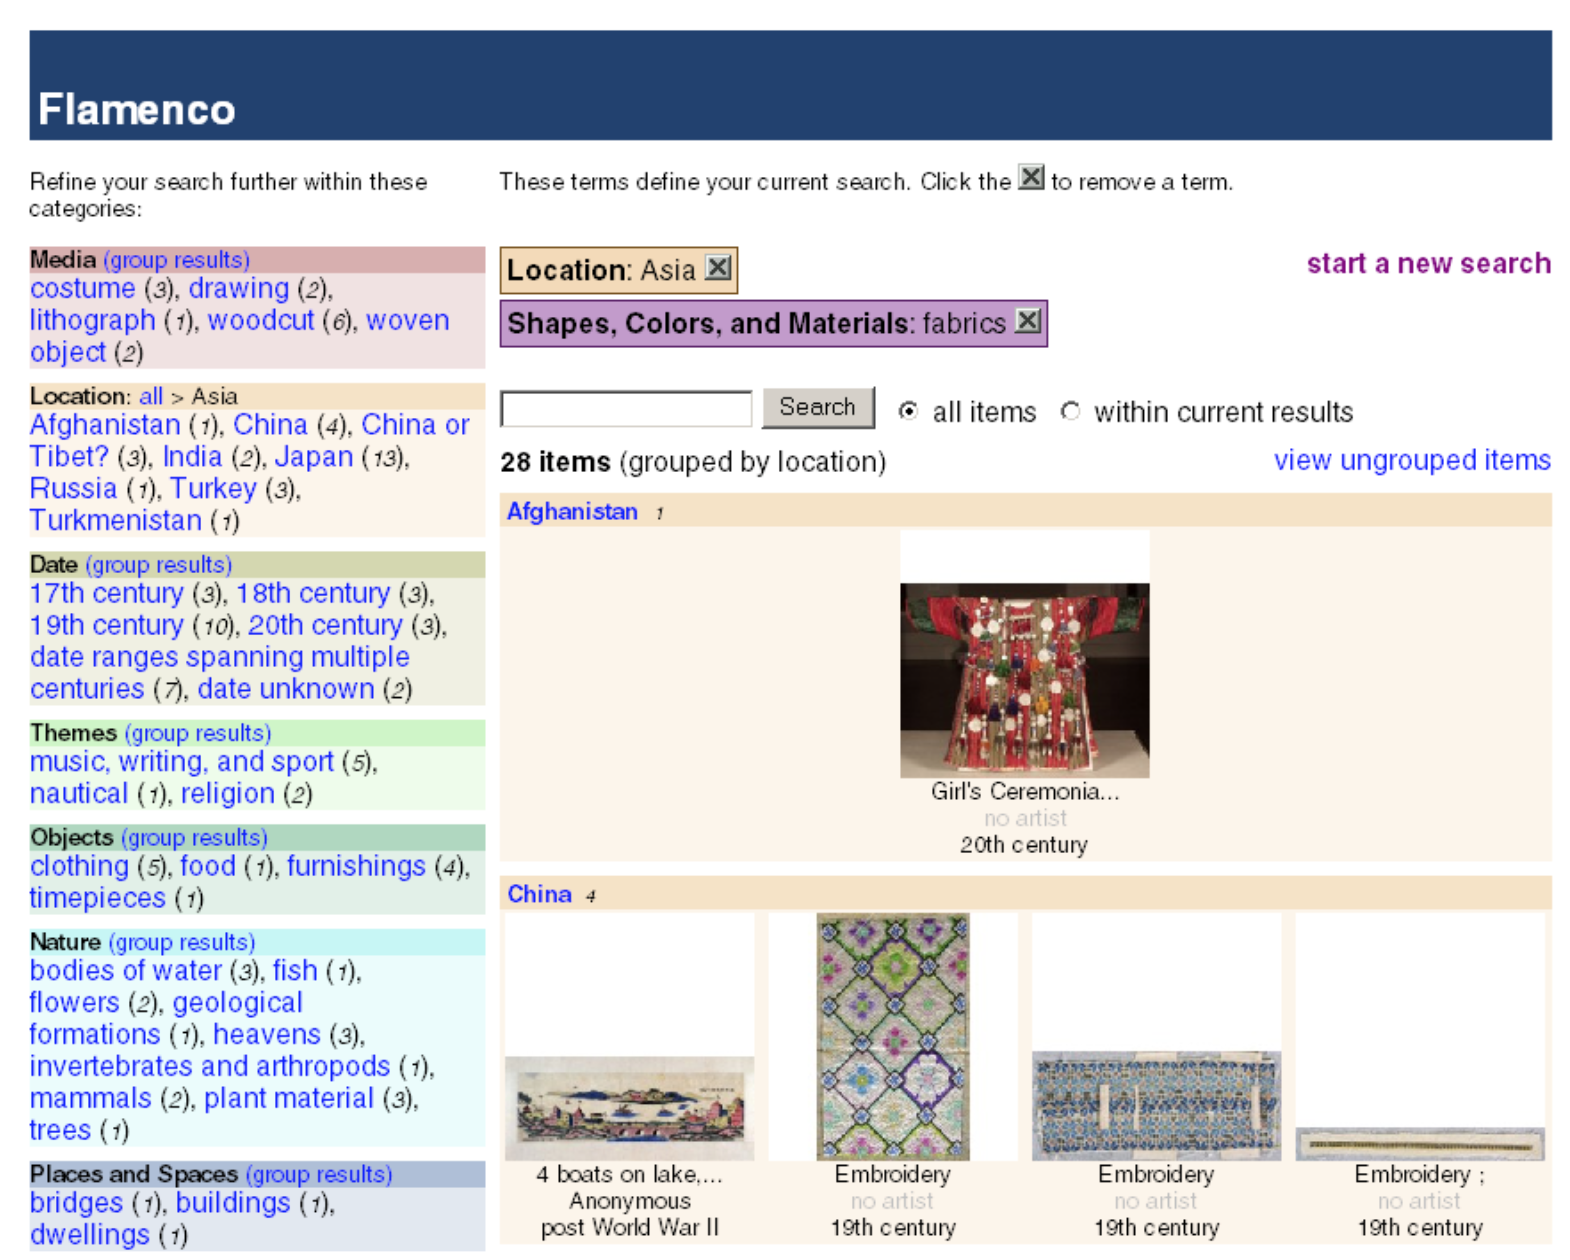
\includegraphics[width=\linewidth]{images/flamenco}
\caption{Flamenco. Only items that are from Asia and made from fabrics are shown. Source: Yee et al. \cite{Yee2003}}
\label{figure:flamenco}
\end{figure*}

This interface is similar to the "local view" on Hasse diagrams presented in Section~\ref{Local View}. The main idea: The dataset comprises several dimensions called \textit{facets}. The user can restrict dimension to certain values. Only items are shown which fulfill the restrictions given by the user. In addition, the user gets suggestion for further restrictions. In Figure~\ref{figure:flamenco}, you can that you see the location is restricted to "Asia" and shapes etc. are restricted to "fabrics". On the left, you can see the suggestions and how many items would be left after restricting. \\

Sacco and Tzitzikas \cite{Sacco2009} say that although \acrshort{fca} and Faceted Search are apparently two distinct approaches to information modeling and access, and they use a different terminology, they are closely related. They also mention that faceted search reduces the cognitive efforts because it ensures that the results are manageable. It feels like, that faceted search is superior to the local view on concepts lattice, if the dataset consist of more than one dimension. So for this reason, the use of FCA for this particular dataset is to question because it actually comprises several dimensions. Nevertheless, the research group applied FCA and it was my task to visualize the results. The interface is described in the next section.

\chapter{Fancy \acrshort{fca} 1.0}
\label{Fancy 1.0}

I start by describing my concept inferred from discussing related work in Section~\ref{Related Work}. Followed by the description of the implementation which can be split into frontend development, responsible for the visual interface in the browser, and backend development, mostly responsible for handling data on the server.

\section{Concept}

The general idea comes from the Virtual Museum of the Pacific discussed in Section~\ref{Museum}. But it had some problem: Missing orientation, missing history of actions and only a rudimentary implemented search interface. I try to address this problems and a schema of the proposed interface can be seen in Figure~\ref{figure:schema}.

\begin{figure*}[!ht]
	\centering
	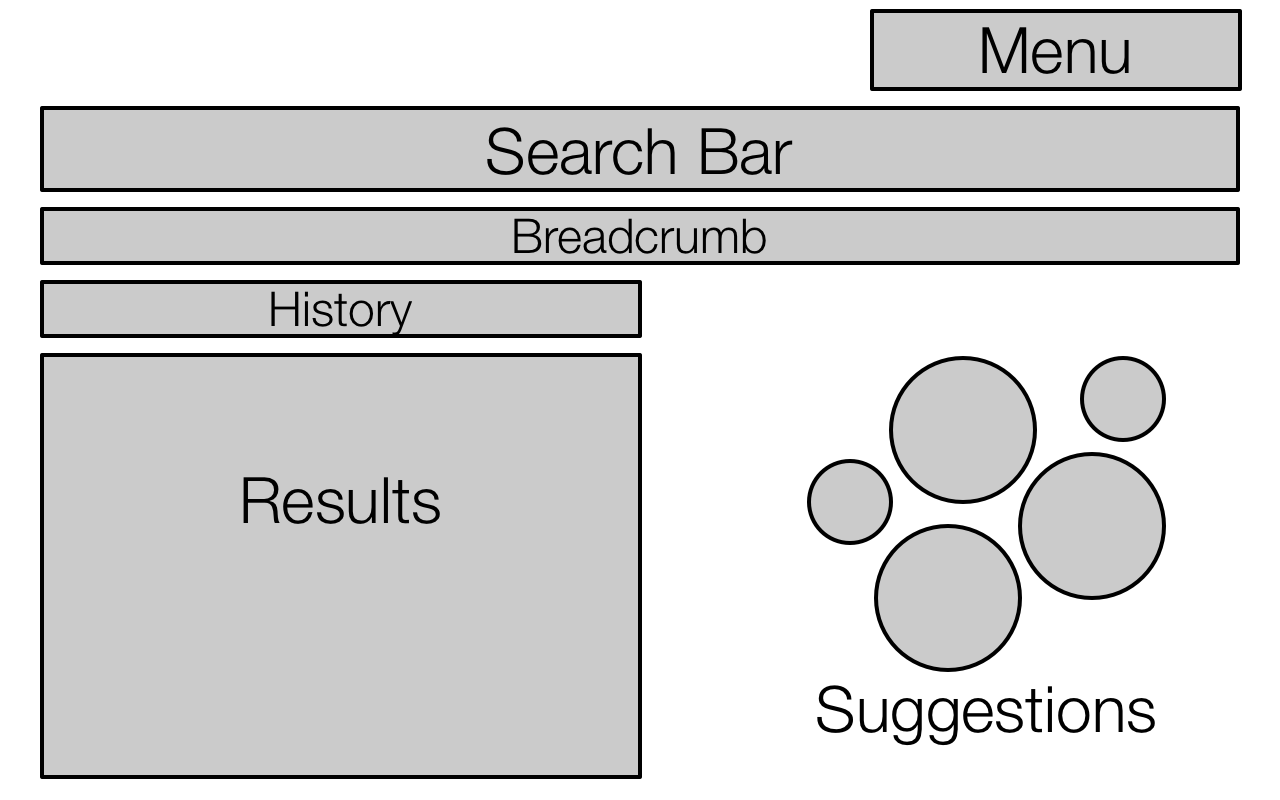
\includegraphics[width=\linewidth]{images/schema}
\caption{Schema of the interface of Fancy FCA 1.0}
\label{figure:schema}
\end{figure*}

First, he interface should remind users of modern search engines: Search bar on top, vertical result list below. Each result has a title with a hyperlinks to a webpage where all the maps are shown in high-quality. Each results has a snippet of the description. The word of the current focus are highlighted. We could not provide thumbnails of the maps because we did not had access to the pictures itself. It was planned to add this feature in later iterations. \\

Second, there was a lack of history of actions or at least orientation. For this we have two functionalities: Breadcrumbs and Navigation History. Breadcrumbs save the current path of search and allow it to easily backtrack. The navigational history tracks the whole session history. The can create an account and login. If he does this, history will be saved even over several sessions. \\

Third, the user can save documents which she found interesting. \\

Fourth, if the user is logged in, all actions, like searches or which linked she clicked on, are logged. They will be saved on the server. This feature was wished by people from the research group to evaluate user behavior. \\

Fifth, the neighboring concepts (the "suggestions") are shown right next to the results as a word cloud. The words are presented in a bubble. The font size and bubble radius depend on the number of documents a formal concept comprises.\\

The UML use case diagram is depicted in Figure~\ref{figure:usecase}.

\begin{figure*}[!ht]
	\centering
	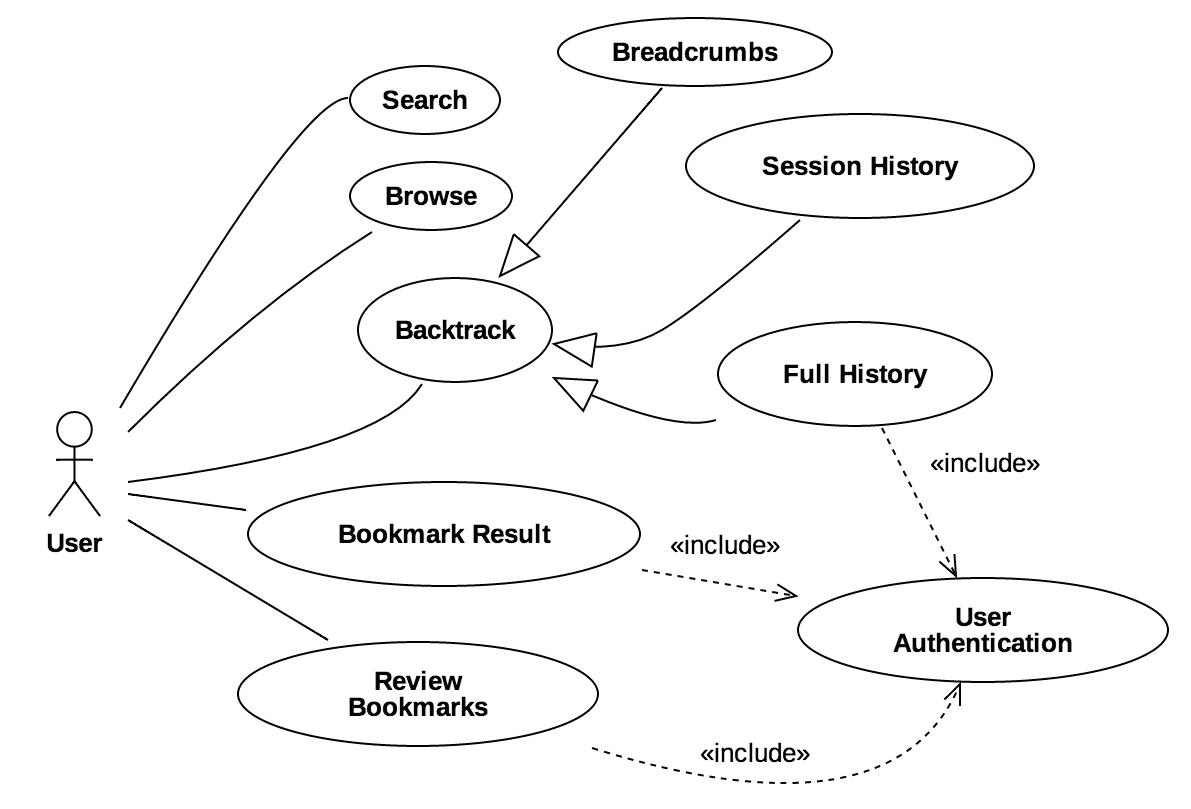
\includegraphics[width=\linewidth]{images/usecase}
\caption{UML use case of Fancy FCA 1.0}
\label{figure:usecase}
\end{figure*}

\section{Frontend}

The interface was implemented with web techniques. So HTML, CSS, Javascript. Instead of writing pure HTML, we use the Jade templating engine \footnote{\url{http://jade-lang.com}}. Instead of writing Javascript, we use CoffeeScript \footnote{\url{http://coffeescript.org}} which compiles to Javascript but offers semantic sugar. For the the word cloud I use D3\footnote{\url{http://d3js.org}} \cite{Bostock2011} as background. D3 utilized SVG to draw elements which are also accessible via the DOM API. The word cloud is a customized graph force-directed layout based on the work from Vallandingham \cite{Vallandingham}. Bootstrap\footnote{\url{http://getbootstrap.com}} adds an overall good look to the site.

\section{Backend}

For the backend, Node.JS with the Express Framework \footnote{\url{http://expressjs.com}} was chosen. Reason one, it is good at handling multiple request in parallel. This is important to handle all the log data. Reason two, I can use the same programming language for frontend and backend: Javascript (CoffeeScript). To save data I use MySQL as database because it was already installed on the server. Because of the use of an Object-relational mapping (ORM) framework, Sequelize \footnote{\url{http://sequelizejs.com}}, it is easily possible to change the database.

\section{Discussion}

The whole implementation has one problem: The data is provided as a JSON file. The clients loads the whole file when he starts the session. All the navigation happens in the frontend. While it is positive, that during the navigation the client does not have to communicate with the server, it is a problem that the client has to deal with over 80 megabytes of data. The server compresses the JSON file to eight megabytes. Downloading this file is acceptable especially in an university environment. But it takes up a lot of memory. The design decision was taken before it was clear that the JSON file would be so huge. This should be addressed in further iterations. \\

That the thumbnails of the maps are not presented is a problem. Albeit all the analysis was done on the metadata, a visual representation would be very useful. \\

The representation of word cloud is relatively arbitrary. This form was chosen to create an interesting interface. It is to question if it is better than a simple table. The table entries decreasingly ordered after the number of documents the formal concept comprises.

\chapter{Evaluation}
\label{Evaluation}

The design of an interface is highly subjective. User studies can help to evaluate an interface but computer scientists are not experts in human studies. For this, a brief review of different techniques for human studies is given first. Then we describe the setup of the study, describe the results and finally conclude. \\

\section{Background}

We will only scratch the surface here. A comprehensive introduction into "Methods for Evaluating Interactive Information Retrieval Systems with User" gives Kelly \cite{Kelly2007}. A shorter introduction gives Hearst in Chapter 2 in her book "User Search Interfaces" . \cite{Hearst2009}.\\

\subsection{Introduction}

So we want to measure usability, but how is it defined? The ISO 9241-11, 1998 \cite{ISO} defines three aspects of usability:
\begin{itemize}
	\item Effectiveness: Accuracy and completeness with which users achieve specified goals.
	\item Efficiency: Resources expended in relation to the accuracy and completeness with which users achieve goals.
	\item Satisfaction: Freedom from discomfort, and positive attitudes towards the use of the product.
\end{itemize}

\subsection{Experiment vs. Evaluation}

It is important to distinguish between the terms 'experiment' and an 'evaluation'. Kelly \cite{Kelly2007} writes:
\begin{quote}
Evaluations are conducted to assess the goodness of a system, interface or interaction technique and can take many forms [..] Experiments have historically been the main method for interactive system evaluation, but experiments can also be conducted to understand behavior [..] Two important characteristics of experiments are that there are at least two things being compared (e.g., system type) and that some manipulation takes place [..] In some types of [interactive information retrieval] studies only a single system is evaluated. This is a weaker form of evaluation since it is not possible to demonstrate how much better users perform or how different their behaviors and inter actions are since there is no point of comparison. Traditional usability tests are examples of this type of evaluation. Traditional usability tests are usually conducted with a single version of a system, with the goal of identifying potential usability problems.	
\end{quote}

In this thesis, the system is only evaluated to find usability problems. No comparison among other systems are conducted but should be done in further investigations.

\subsection{Informal Usability Testing}

Hearst \cite{Hearst2009} describes Informal Usability Testing as "Showing designs to participants and recording their responses". It is often used in short iterative cycles to quickly evaluate a design. \\

 We conduct informal usability studies because we do not have proper equipment nor any experience with user studies.

\subsection{Questionnaires}

A questionnaire comprises a set of questions and is cheap and fast way to gather information from people. Kelly et al. \cite{Kelly2008} describe two types of questions as follows:

\begin{quote}
	Questionnaires can be comprised of closed questions, open questions or a mixture of both. \textit{Closed questions} are questions that provide a fixed set of responses with which subjects must respond. It is common practice for usability questionnaires to include closed questions in the form of statements such as, the system was easy to learn to use. Subjects are typically provided with 5–7-point Likert-type scales for responding, where one scale end-point represents strong agreement and the other represents strong disagreement. [..] \textit{Open questions}, on the other hand, do not provide a response set and subjects are able to provide any type of response they feel is appropriate. 
	\end{quote}


\subsection{Thinking Aloud}

Kelly \cite{Kelly2007} writes by referring to Ericsson and Simon \cite{Ericsson1993}: "The think-aloud method asks subjects to articulate their thinking and decision-making as they engage in [interactive information retrieval]". The comments from the participants have to be collected. Either by recording the session or by taking notes. It is hoped that the conductors can learn from the thinking process of the participant. There exist variations of this techniques. Because it can be exhausting, challenging and awkward to talk to yourself all the time, participants are encouraged to report either at some fixed times or when the feel the need.

\section{Setup}

The evaluation was done with five people with a background in humanities. First, an introductory presentation was given in Spanish. Then they were split into two groups. Each group interacted with the interface. The people in the group rotated. There were three tasks they should do. The participants were encouraged to talk aloud. Sometimes the instructions asked them what they are doing or what they feel. The one group was recored with an iPhone 6 Plus\footnote{\url{https://www.apple.com/iphone-6}}. The session of the other group was not recored and could not be evaluated at all. After they session they had to fill in a pen-and-paper questionnaire. We use ten closed questions from the USE questionnaire \cite{lund2001measuring} and four commonly asked open questions as asked by Kelly \cite{Kelly2008}. They can found in appendix \ref{app:open} and \ref{app:closed}. The participants wrote in Spanish which was translated afterwards.

\section{Results}

We group thinking aloud, remarks and open questions together because the comments were very similar. After that, we present the results of the closed questions.

\subsection{Thinking Aloud, Remarks and Open Questions}
It turned out, that the evaluation was also a evaluation of the whole research project. All participants mentioned that the interface does not suite their needs. All wanted to refine the search by location and time range and map creators. \acrshort{fca} cannot provide this kind of functionality.\\

Several participants gave advise how to improve the result list. First, shorten the snippets so that they could read more titles. This could be done by restricting the text length and offering a "show more" button. Second, they mentioned that the thumbnail should be added. \\

Overall, they give positive comments regarding the interface. They found the navigation with the breadcrumb helpful. \\

They were not interested in the "Bookmark" feature. Maybe it was because it was an artificial meeting and not a real work environment. They found it a good idea to link to the original site. \\

There were some problems. They were irritated that they could not search for arbitrary terms. Word for instance like "Valencia" were not in the collection and so also not in the lattice. It was for them not clear that the terms has to be decided before. They suggested that this should get fixed. \\

They search interface was not used very often. They used the bubble cloud to navigate through the lattice. \\

One participant mentions that he wanted the see related field to a given field. This would be helpful for his research. \acrshort{fca} can easily provide this method and it is a fail in the interface that it was not included.\\

\subsection{Closed Questions}

Out of the five participants only three filled out the questionnaire. The results are in the annex \ref{app:closed}. The results correspond to the comments made by participants. The weakest results got the sentences "It meets my needs" and "It does everything I would expect it to do". The best result got the sentence "It is easy to use".

\section{Accessibility Analysis}

In addition to the the evaluation with users, there was a evaluation regarding accessibility features. It was conducted by people from the UNED: Miguel Angel Marqueta and Covadonga Rodrigo San Juan. It can be found in appendix \ref{app:access}. They comments were overall positive buy they highlighted some problems with the interface: It is possible to zoom in the bubble cloud, but there are no buttons on the screen for it. In the current state, the zooming can only be done with a mouse or a touchpad. 

\section{Conclusions}

 Zobel \cite{Zobel2004} proclaims: "Far too many human studies in computer science are amateurish and invalid" and with this study we proved him true. They overall setup was improvised and all instructors had no experience with user studies. Even though it cannot stand scientific standards, it is useful as informal evaluation. \\
 
 We can conclude that \acrshort{fca} for this collection in the current implementation is useless. It cannot over the separation between location or time ranges. It looks like that for faceted search as described in Section~\ref{dyafs} promises better results. \\
 
 It also suffers from the fact, that only a limited number of terms was selected to built up the concept lattice. If the users searched for terms wich were presented in the documents, they could not explain it why they got no results back. It is impossible to create a concept lattice from all words uses in the documents. It could be promising to combine searching with FCA liked it was done in other systems as described in \ref{Local View}. Implement and ordinary search and built up a concept lattice from the results. \\
 
 For the interface itself, it looks like they liked it. Even though there are some problems like the result list which should be addressed. \\
 
 After this demolishing results, it was decided not to pursue the idea of FCA for the collection of maps. But the tool itself looks promising that why I transform the tool to visualize arbritary concept lattices. The changes are described in the following section.
 
\chapter{Fancy \acrshort{fca} 2.0}
\label{Fancy 2.0}

\blindtext

\chapter{Conclusions}
\label{Conclusions}

\blindtext

\newpage
\bibliographystyle{plain}
\bibliography{biblography}

\listoffigures
\listoftables 


\newpage
\appendix
\chapter{Appendix: Accessibility Report}
\label{app:access}

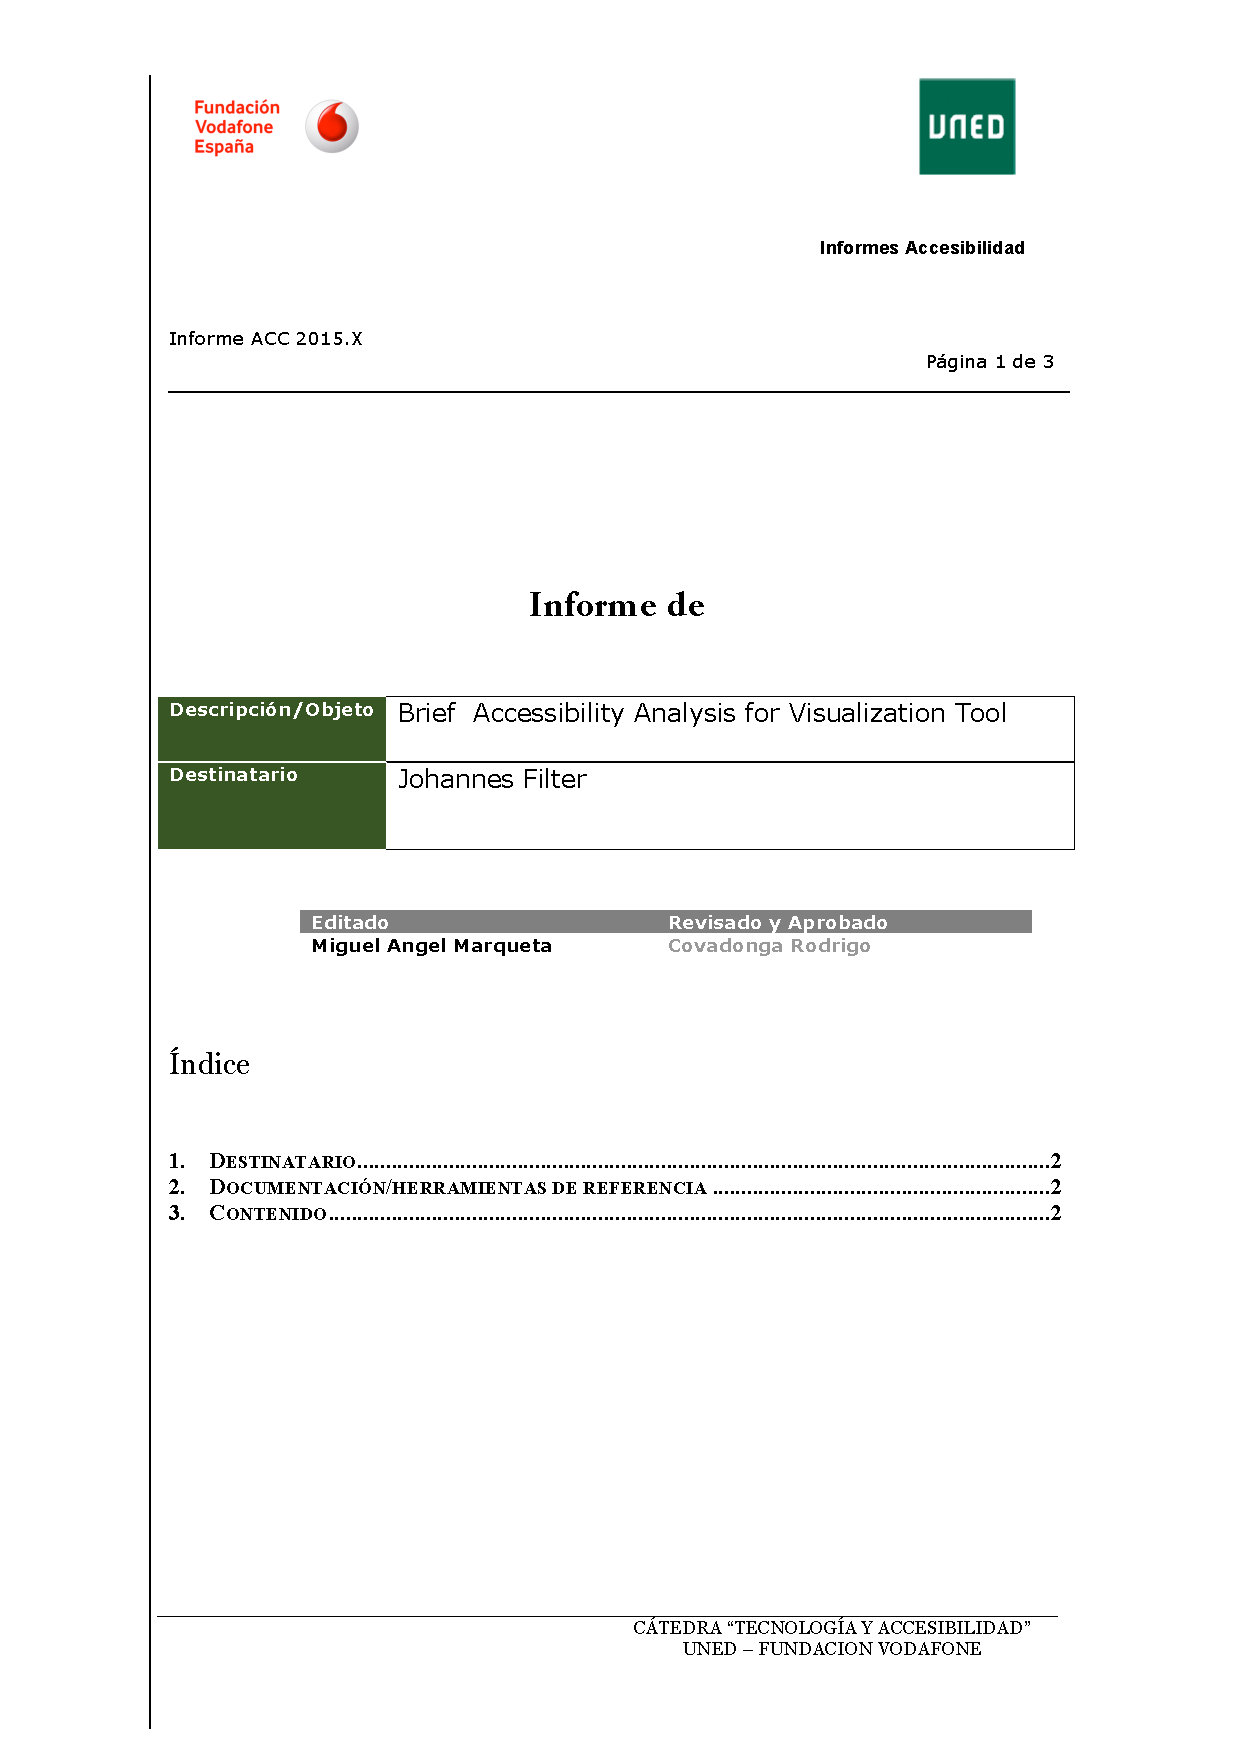
\includepdf[pages={-}]{appendix/report.pdf}

\chapter{Appendix: Closed Questions}
\label{app:closed}

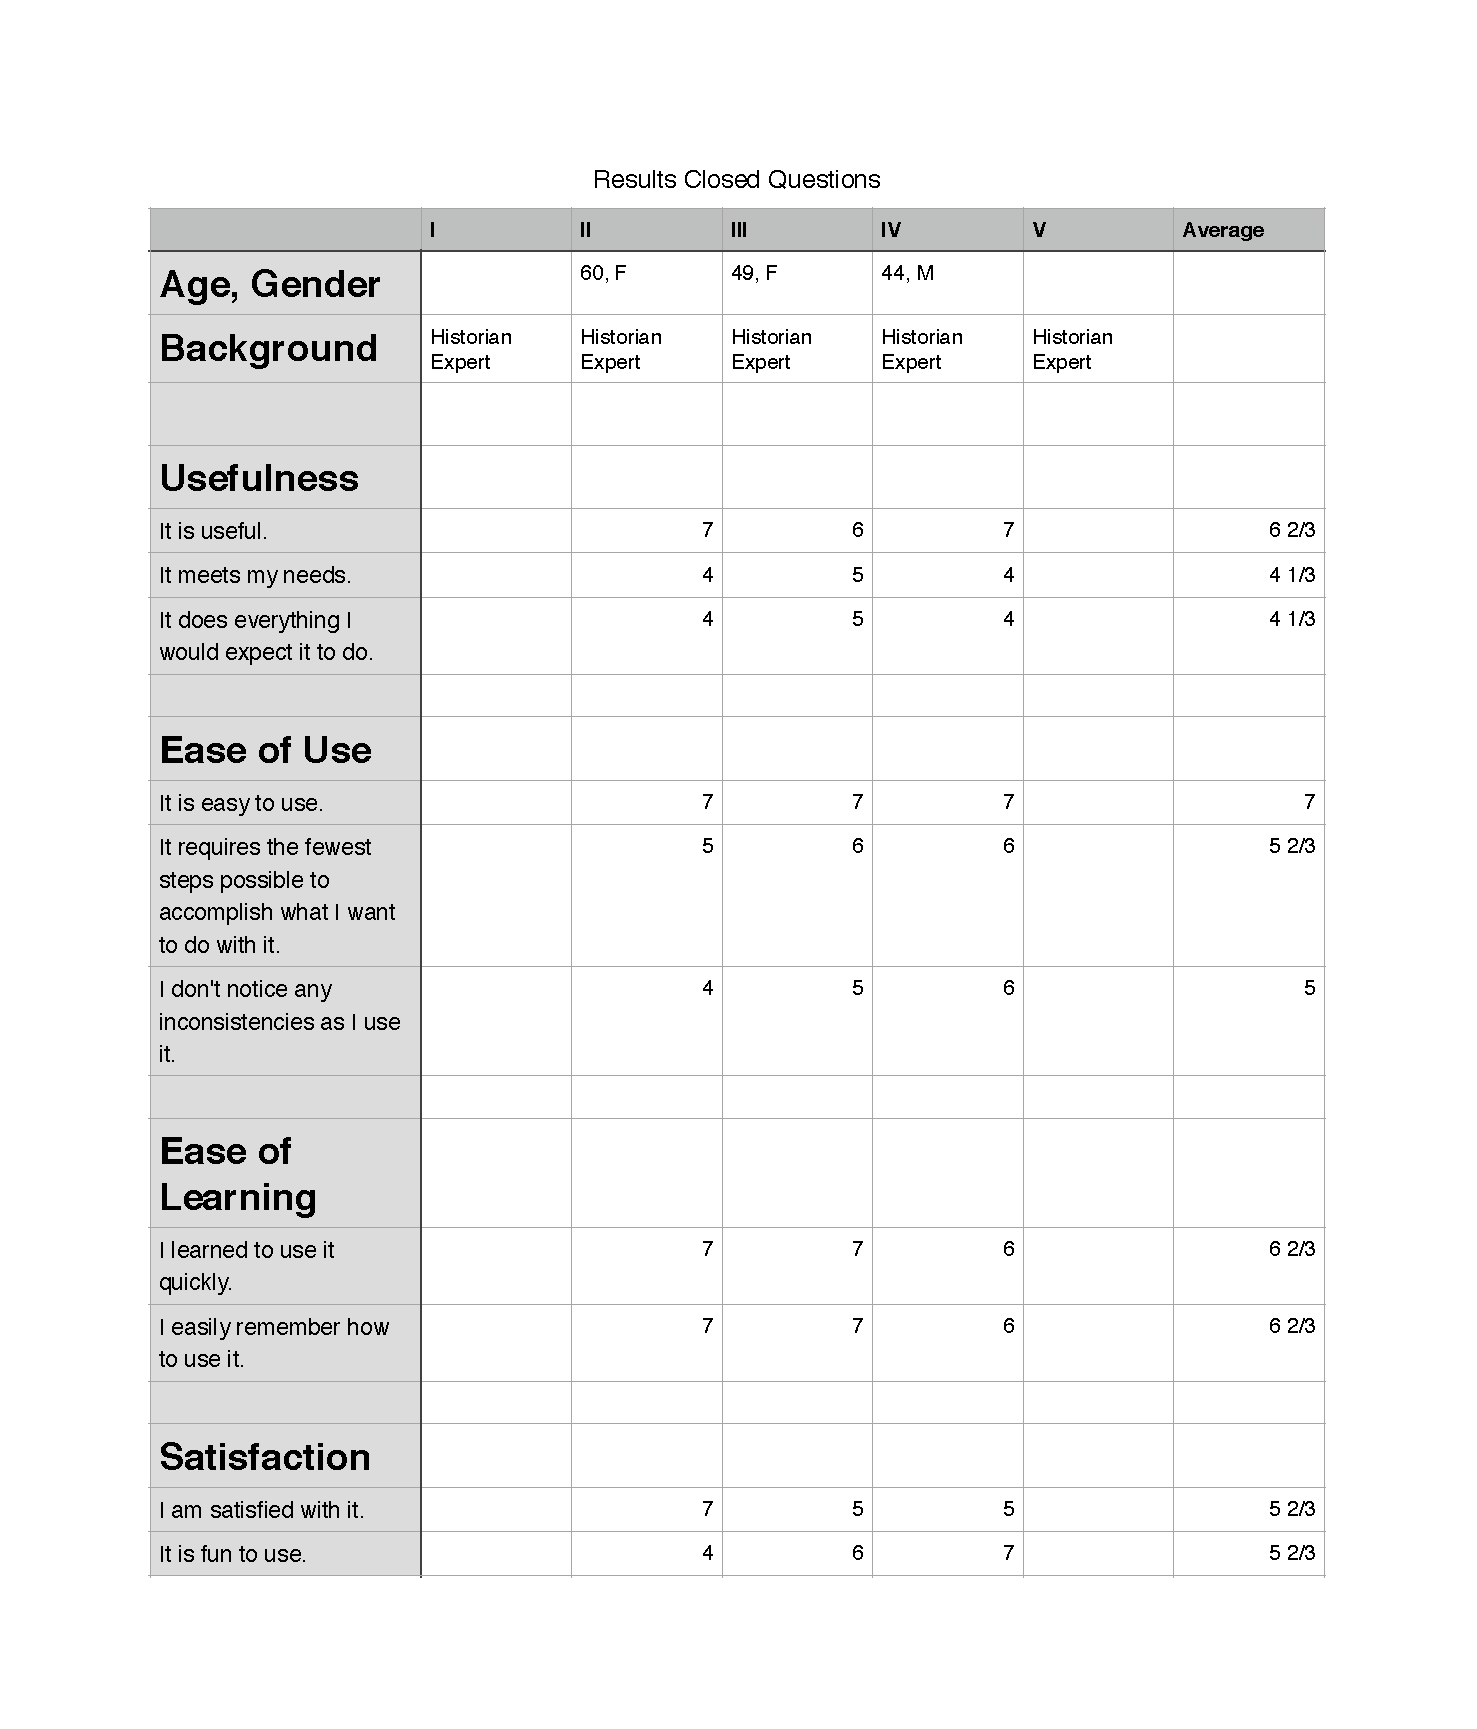
\includepdf[pages={-}]{appendix/closed.pdf}

\chapter{Appendix: Open Questions}
\label{app:open}

\begin{itemize}
	\item What were the most positive things about using this system and why?
	\item What were the most negative things about using this system and why?
	\item How would you improve this system and why?
	\item Is there anything else that you would like to tell us about this system and your experiences using it?
	\item In comparison with other systems (Interface of Catálogo Colectivo de las colecciones de Mapas and previous work of this research group).
Do you think it is more useful? If yes, which part of the system is more useful.
\end{itemize}


\end{document}